\documentclass[a4paper,man,floatsintext,natbib]{apa6}

\usepackage[english]{babel}
\usepackage[utf8x]{inputenc}
\usepackage{float}
\usepackage{amsmath}
\usepackage{graphicx}
\usepackage[colorinlistoftodos]{todonotes}
\usepackage{natbib}
\usepackage{subcaption}
\usepackage{pdfpages}
\usepackage{hyperref}
\usepackage{comment}

\hypersetup{
	colorlinks=true,
	linkcolor=black,
	citecolor=black,
	urlcolor=black
}

\definecolor{Blue}{RGB}{0,0,255}
\definecolor{Green}{RGB}{10,200,100}
\definecolor{Red}{RGB}{255,0,0}
\definecolor{Orange}{RGB}{255,140,0}
\newcommand{\jd}[1]{\textcolor{Blue}{[jd: #1]}}  
\newcommand{\ek}[1]{\textcolor{Orange}{[ek: #1]}} 

\newcommand{\tableref}[1]{Table \ref{#1}}
\newcommand{\figref}[1]{Figure~\ref{#1}}
\newcommand{\appref}[1]{Appendix \ref{#1}}
\newcommand{\sectionref}[1]{Section \ref{#1}}

\title{\large Pick the Yellow ... Strawberry? Production Expectations Explain Variation in Contrastive Inference}
\shorttitle{An RSA account of contrastive inference}
\author{Elisa Kreiss, Judith Degen}
\affiliation{Stanford University}

\begin{document}

\maketitle


\section{Introduction}\label{sec:intro}

% \ek{clarify what you call item, object, type.}


% \ek{what is the value of studying contrastive inference? -- investigating perspective-taking, online processing, pragmatic vs lexical debates}


Communication generally involves a \emph{speaker} who sends out a communicative signal (e.g., speaks or signs a phrase, draws a picture, or points to an object), and a \emph{listener} who perceives that signal and tries to understand its meaning. For example, if a speaker says ``Pick up the yellow banana!'', a listener can easily pick out the top left object in \figref{example-contexts}A as the speaker's intended referent. 
A key feature of (human) communication is that listeners incorporate information as soon as it becomes available. For instance, when listeners have so far only heard ``Pick up the yellow...'', they already disregard the two non-yellow objects in the display because those are incompatible with the information received at that point \citep{Tanenhaus:1995,Sedivy:1999}. 

\begin{figure}
	\begin{center}
		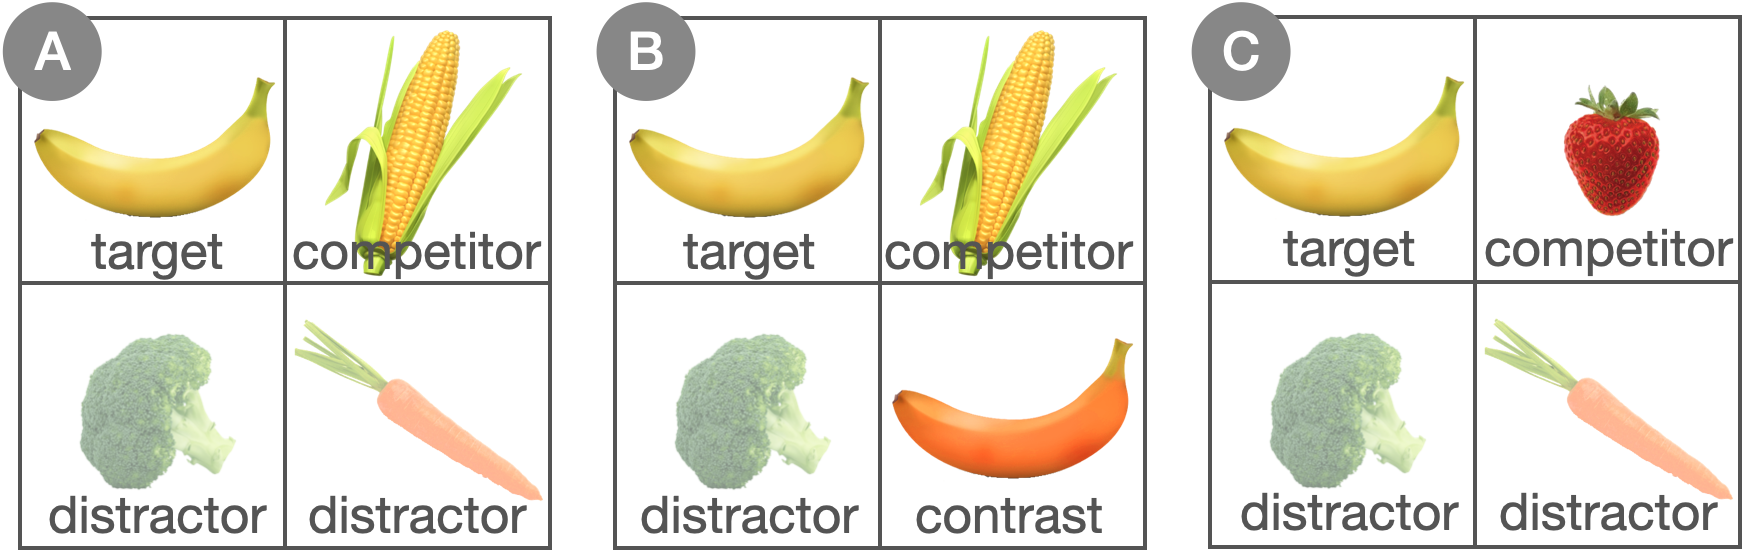
\includegraphics[width=.8\textwidth]{img/example-contexts.png}
	\end{center}
\caption{Three contexts of objects.} 
\label{example-contexts}
\end{figure}

Moreover, listeners leverage contextual information to draw pragmatic inferences about the object the speaker is most likely referring to \ek{decide on which work to cite here}. While listeners don't show a preference for neither the yellow banana (the \emph{target}) nor the yellow corncob (the \emph{color competitor}) in \figref{example-contexts}A, this changes as soon as a differently colored banana is introduced (as shown in \figref{example-contexts}B). Again upon hearing ``Pick up the yellow...'', listeners now already show a preference for the banana over the corncob \citep{Sedivy:1999,Sedivy:2003,Aparicio:2016,Rubio-Fernandez:2019}. Since the original findings in the size adjective domain \citep{Sedivy:1999}, this pattern of preference has been referred to as the \emph{contrast effect} or \emph{contrastive inference}.

It is important to distinguish three concepts here: \textit{preference}, \textit{inference}, and \textit{contrastive inference}. \emph{Preference} describes listeners' behavioral data that shows which objects are currently considered as most likely referents. This can be evidenced for example by listeners' increased fixations of an object \citep{Tanenhaus:1995,Eberhard:1995}. An \emph{inference} here describes any change in preference that is not due to changes in truth-conditions. For example, the target can already be uniquely identified after ``Click on the yellow...'' if the yellow corncob is replaced by a red strawberry (see \figref{example-contexts}C). The resulting boost in target preference is therefore not due to an inference. In comparison, if we exchange one of the distractors for an orange banana (see \figref{example-contexts}B), target preference increases even though target and competitor are still the only possible referents. This change in target preference is therefore an example of \emph{inference}. We call it a \emph{contrastive inference} because the target preference increases due to the introduction of a contrast (here the orange banana).

% But what are listeners doing here? 
% A purely lexical (or \emph{form-based}) account would suggest that contrastive inference arises because size adjectives are generally considered to require a comparison class, such as a small glass, to be evaluated. However that the effect has been found with material adjectives, which are generally considered not to require a comparison class, speaks against it \citep{Sedivy:2003}. 
To explain how listeners draw this rapid contrastive inference, \cite{Sedivy:2003} proposes that it arises from listeners' pragmatic reasoning about the informativity of an utterance. Following the Maxim of Quantity \citep{Grice:1975}, a cooperative speaker can be expected to not include more information than necessary into their utterance. In \figref{example-contexts}B, listeners can therefore reason that the speaker could have referred to the corncob more simply as \textit{the corncob}. According to this account, the use of a modifier to refer to the corncob would be considered \emph{descriptive} and should not result in an inference. Instead, including the modifier is only necessary to distinguish the yellow from the orange banana. Here, the modifier is used in its contrastive function. Since the contrastive use of the modifier is considered more informative than the descriptive one, listeners interpret the modifier contrastively whenever possible. This reasoning predicts a preference for the target when a contrast is present (\figref{example-contexts}B) and no preference when the contrast is absent (\figref{example-contexts}A).
% By introducing an orange banana, listeners can apply the following reasoning: If the speaker is being cooperative, we expect them to not include more information than necessary — so they could have referred to the pitcher more simply as just “the pitcher” and the adjective is only necessary for distinguishing the tall from the short glass (which is why it receives the contrastive interpretation) (following Grice Maxim of Quantity; see Grodner for a nice discussion of lexical vs. pragmatic effect). \citep{Grodner:2011}

% This account faces the challenge to explain what makes the inclusion of the modifier more informative than the bare form \citep{Grodner:2011}. This is achieved by assuming that adjectives are generally descriptive, but can take on a more informative contrastive role. For example, \textit{yellow} fulfills a contrastive purpose when referring to the banana in \figref{example-contexts}B, because it's differentiating it from the orange banana. However when \textit{yellow} is used to refer to the banana in \figref{example-contexts}, it is simply a feature that describes the object. Whenever available, the contrastive interpretation is preferred over the descriptive one, since it is more informative and therefore contrastive inference arises.

% According to this account, a listener needs to decide for each occurrence of \textit{tall} whether it receives a descriptive or contrastive interpretation. \citeauthor{Sedivy:1999} argues that whenever a contrast is available, the contrastive interpretation is activated due to the informativity constraint as outlined above (taken from \cite{Grodner:2011}).
% In \ek{Figure 1A}, the speaker assigns to \textit{tall} the descriptive interpretation, since there is neither a small glass nor a small pitcher. In \ek{Figure 1B}, \textit{tall} can be interpreted descriptively when referring to the competitor, and contrastively when referring to the target. The listener prefers the contrastive over the descriptive interpretation because it is a more informative use of the modifier and therefore the target is preferred over the competitor.

In order to make this prediction, this account needs to postulate three central assumptions. Firstly, the speaker needs to be considered cooperative for the inference to occur \citep{Grodner:2011}. Secondly, adjectives can take on two separate roles (\emph{descriptive} and \emph{contrastive}). Thirdly, the use of an adjective in its contrastive function is more informative than when it's used descriptively. Finally, descriptive adjective use does not trigger any target inference.
While previous literature appears to confirm that when a speaker is perceived as uncooperative, contrastive inference does not arise \citep{Grodner:2011,Ryskin:2019}, none of the other assumptions has previously been tested.

Furthermore, some previous empirical results are at odds with this account of contrastive inference. In a series of studies investigating contrastive inference in the color adjective domain, the contrast effect appeared less stable than predicted under this account. \cite{Sedivy:2003} reports that the contrastive inference arises in contexts where the target object has a predictable color (such as the yellow banana in \figref{example-contexts}) but not when it is replaced by an object with an unpredictable color like a cup, which comes in many colors.
She shows that these objects differ in how likely a speaker is to produce the color modifier for the object in isolation: in the absence of a contrast, a yellow banana is usually called \textit{the banana} while a yellow cup is often called \textit{the yellow cup}, which \citeauthor{Sedivy:2003} calls these objects' \emph{default descriptions}. To account for this finding, she extends the contrastive inference account by another assumption: Only in cases where the modifier is not part of the default description is its observation surprising and the adjective's contrastive function is inferred. If its observation is not surprising, listeners simply accept the adjective in its descriptive function.\\
At the same time, \cite{Sedivy:2003} also finds that when using yellow banana-like items as targets and yellow cup-like items as competitors, listeners prefer the cup (the competitor) over the banana (the target) even if no contrast is present\footnote{This surprising finding is mentioned in footnote 5 in \cite{Sedivy:2003}.}. This is a puzzle for any account of contrastive inference so far.

% Crucially they also assume that descriptive use of a modifier does not result in an inference (it might maximally be used to make speaker appear unreliable and gets rid of all inferences \citep{Grodner:2011,Ryskin:2019}).



% \ek{Main points that should come out of the introduction:}\\
% - target preference, target inference, contrastive inference\\
% - explanation of the paradigm\\
% % - why is it useful as a paradigm (which questions are addressed)\\
% - our contributions:\\
% - empirical evidence of within adjective class variation of contrastive inference (some evidence of binary variation in Sedivy; other than that only variation between lexical categories (Aparicio, RF, Heller2020,...))\\
% - first computational model that makes quantitative predictions about target inference and therefore contrastive inference. It doesn't distinguish between different causes why a speaker might use a modifier which is why it only makes smushed predictions. variation -- when it should vary given a rational agent\\
% - doesn't directly make predictions about contrastive inference but target inference\\
% - nonbinary predictions\\
% - fully pragmatic model that makes descriptive/contrastive distinction obsolete\\
% - not only the target, but also the competitor matters\\
% - prior beliefs again change contrastive inference which cannot be predicted by any form-based accounts\\
% - we can change the size of target boost/competitor reduction within the color domain, calling into question generalized statements about color-adjective CI behavior

In this paper, we propose a highly speaker-centric account of contrastive inference which is based in the Rational Speech Act framework \citep{Frank:2012,Goodman:2016}. In contrast to previous accounts, this model makes predictions only on the assumption of speaker cooperativity and listeners reasoning about speakers' most likely utterances. We will show that this leads to new predictions of contrastive inference that cannot be explained by other accounts without violating at least one of their underlying assumptions. Furthermore as to our knowledge, it is the first account of contrastive inference that makes \emph{quantitative} predictions on how likely a listener is to prefer the target over the competitor when a contrast is absent and present. From that we can derive the boost in target preference that is due to the presence of a contrast. It allows us to abstract away from specific factors that can affect interpretation (such as adjective classes, descriptive vs. contrastive interpretation, or salience) by only considering production and prior probabilities. 
% \ek{contrastive inference is not this thing that arises from a listener realizing that they need to use the contrastive over the descriptive interpretation. It is simply one of many inference changes all originating from very gradient and probabilistic production expectations}


% This model is the first account of contrastive inference that makes quantitative predictions of target preference and therefore contrastive inference. It lets us abstract away from specific factors that can affect interpretation and only considers production and prior probabilities. Assuming a flat prior, we find that we don't have to introduce any additional linguistic and cognitive factors to explain contrastive inference behavior. Simply from production expectations alone, we can derive the patterns in interpretation, indicating that production and comprehension are closely linked. The model also makes one more prediction: In addition to production probabilities, the prior probabilities of an item being referred to should affect the inferences drawn. This has been shown in several other domains such as \ek{cite Tessler, Degen,...}. We show that introducing prior speaker preferences affects listeners' interpretations, suggesting that just like other pragmatic inferences, contrastive inferences are highly dependent on the broader context (e.g., speaker specificity, world knowledge). However even though the effects are in the direction predicted by the model, there are interesting discrepancies which might hint at shortcomings of how the prior is defined in RSA.

We show that this model closely predicts listeners' inferences using color adjectives without assuming any additional linguistic and cognitive factors. Simply from production expectations alone, we can derive the patterns in interpretation, indicating that production and comprehension are closely linked. Motivated by the model predictions, we provide empirical evidence that not only the target, but also the competitor matters for eliciting contrastive inference. By changing whether a speaker is expected to produce an adjective for the target and competitor, we find high variation of target preference/inference within the color domain, which calls into question generalized statements about color-adjective inference patterns. Furthermore, our results suggest that listeners' interpretations are also affected by their prior beliefs about what the speaker is most likely referring to, making contrastive inference more malleable to previous exchange than is predicted by other accounts and discussed in the literature.



\section{A Bayesian account of contrastive inference}

The Rational Speech Act framework \citep{Frank:2012,Goodman:2016} is a probabilistic (and thus non-deterministic) Bayesian account of natural language which ascribes a central role to the speaker in pragmatic interpretation. The core idea of the model is that a listener and a speaker recursively reason about each other: A pragmatic listener $L_1$ wants to infer the meaning of an utterance $u$, as formulated by the pragmatic speaker $S_1$. Possible referents $r$ are assigned a probability proportional to the probability that $S_1$ will produce $u$ to convey $r$ multiplied by the listener's prior belief in $r$ $P(r)$, as defined by Bayes' Rule.\footnote{The pragmatic speaker model and further recursive steps are spelled out in detail elsewhere \citep{Goodman:2016}. Since we will elicit speaker probabilities empirically, we need not be concerned with the details of the speaker model.}

\begin{equation}
	P_{L_1}(r|u) \propto P_{S_1}(u|r) * P(r)
\label{eq-prior}
\end{equation}

To simplify the following example, we will assume that listeners have a uniform prior $P(r)$ over all objects in the display\footnote{The simplifying assumption is justified by the results of Exp.~2.}. Then the RSA model predicts a direct relationship between the production probabilities $P_{S_1}$ and the listener's distribution over possible referents $P_{L_1}$.

While RSA has typically been applied to the analysis of full utterances, it can straightforwardly be extended to generate predictions at the sub-sentential level\footnote{One exception is the Incremental Iterated Response Model of Pragmatics, which is also shown to qualitatively predict contrastive inference in general \cite{Cohn-Gordon:2019}.}. To generate RSA predictions for an incomplete referring expression such as \textit{Click on the yellow...}, we take $P_{S_1}$ to correspond to the contextual probability of color mention for each referent in the display. This corresponds to marginalizing over the probabilities of all continuations of the utterance (i.e., \textit{Click on the yellow banana/corncob/lettuce/...!}). Let's investigate this account's qualitative predictions:

\begin{figure}
	\begin{center}
		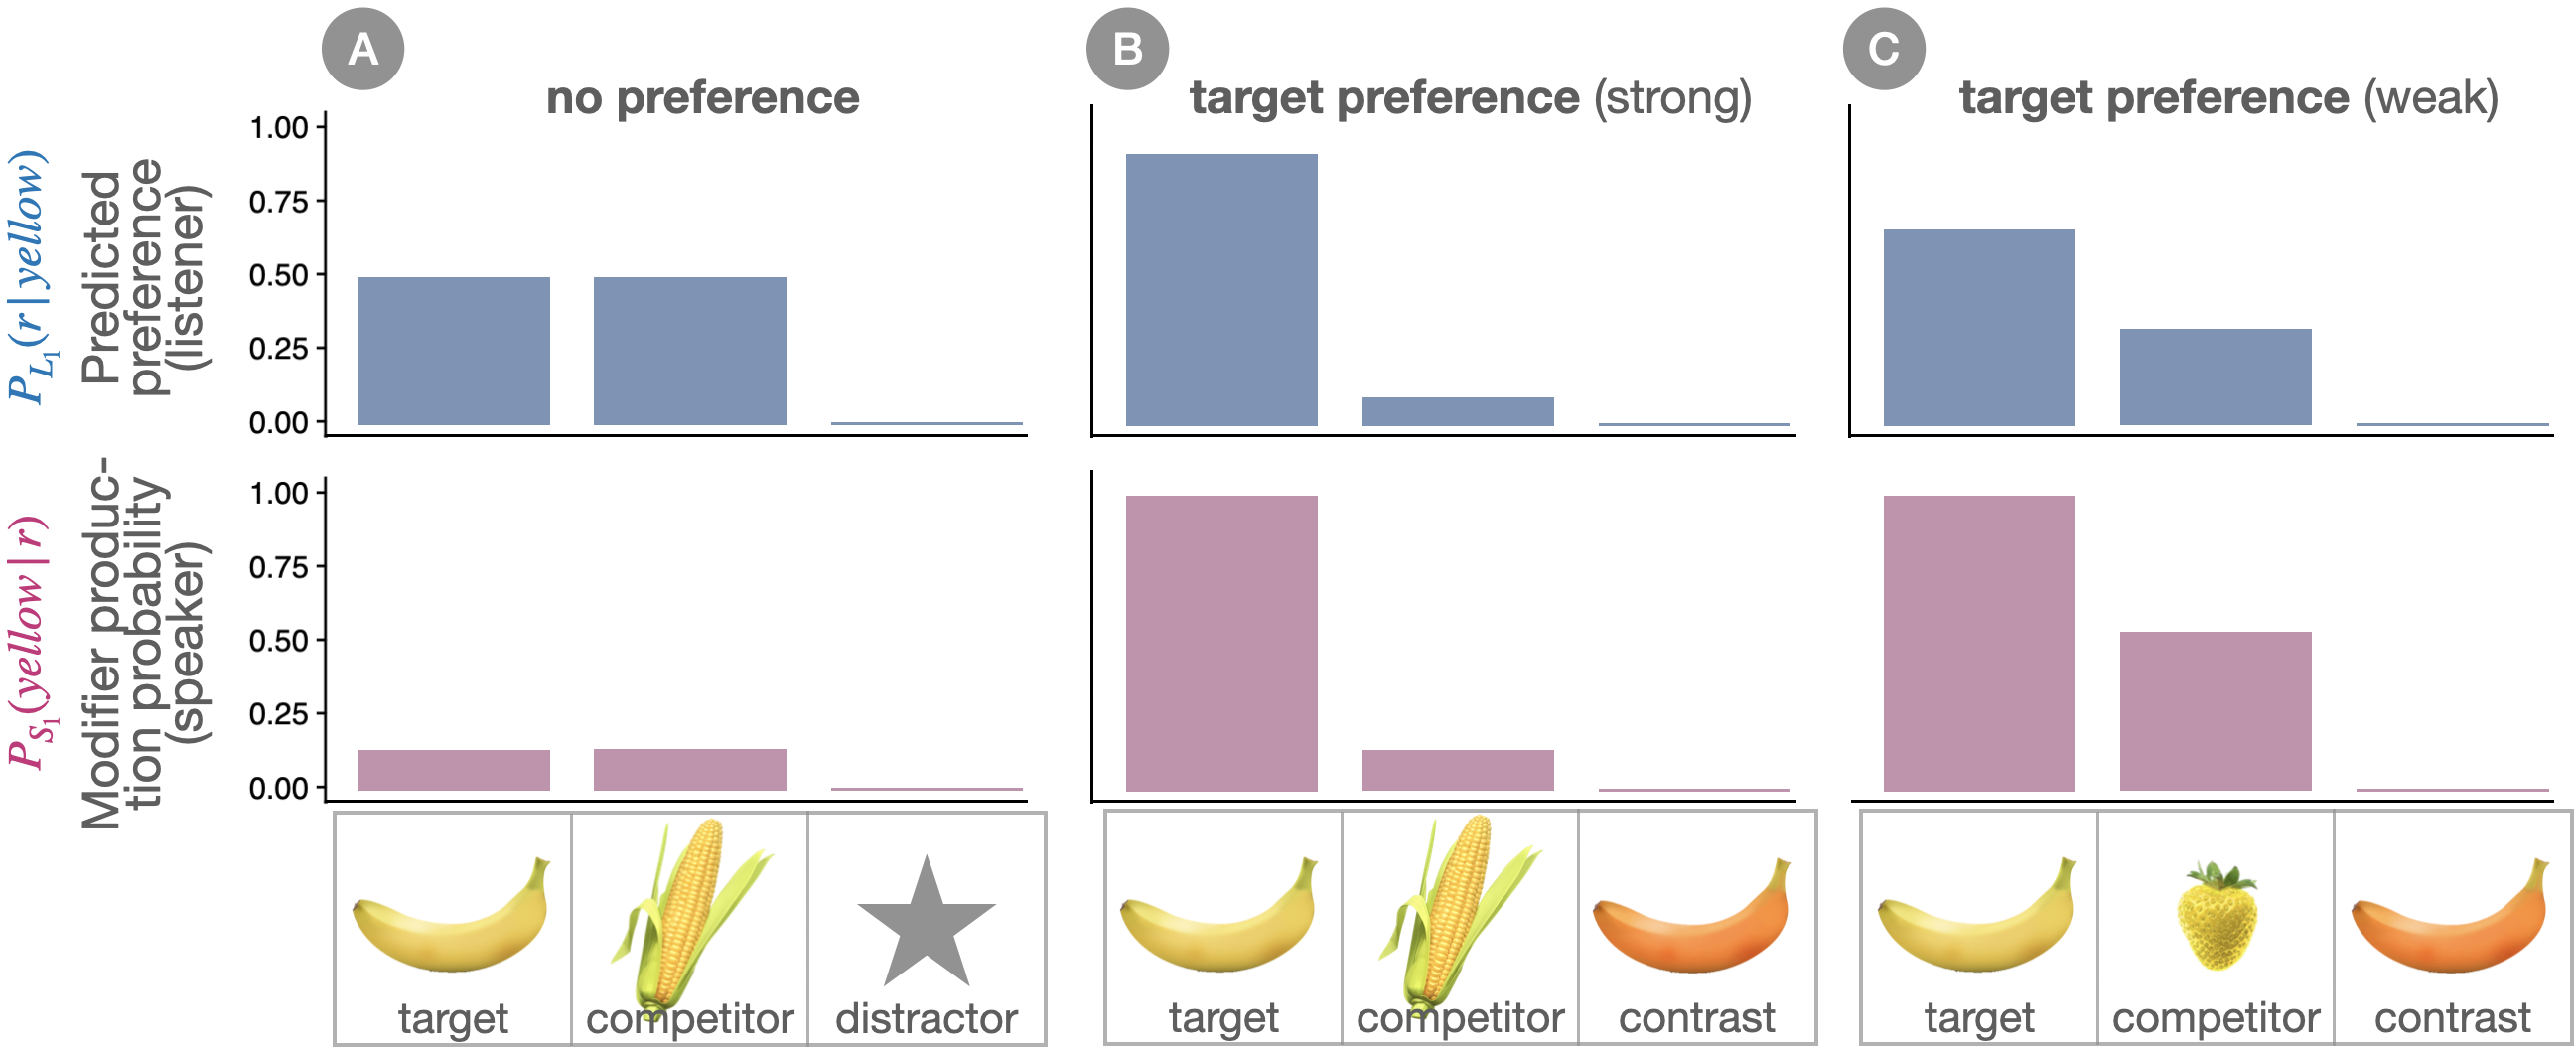
\includegraphics[width=1\textwidth]{img/rsa-example.png}
	\end{center}
\caption{Qualitative RSA predictions.} 
\label{rsa-example}
\end{figure}

Consider the example contexts in \figref{rsa-example}A and \figref{rsa-example}B. Upon hearing the modifier \textit{yellow}, the pragmatic listener $P_{L_1}$ considers how likely a speaker is to include this modifier in their referring expression for each object in the display. Since only the target (yellow banana) and the competitor (corncob) are yellow, we assume that the production probabilities of \textit{yellow} for the other objects in the display are 0. This only leaves the target and the competitor as potential referents. 

Hypothetical modifier production probabilities for target and competitor are shown in the middle row of \figref{rsa-example}. 
Assume that in the absence of a contrast object (\figref{rsa-example}A), speakers are equally unlikely to include the color modifier when referring to the target banana (probability 0.1) and its color competitor, the corncob (0.1). Pragmatic listener predictions are obtained by renormalizing these probabilities, resulting in a target preference of 0.5, i.e., the pragmatic listener does not prefer one potential referent over the other.

Does RSA predict the target preference and therefore contrastive inference in context \figref{rsa-example}B? Assuming that the presence of the contrasting orange banana does not affect the speaker's modifier production probability for the competitor corncob but does increase modifier production probability for the target banana to 0.9, renormalizing the production probabilities results in a target preference of 0.9. This way RSA can reproduce the classic contrastive inference pattern without assuming a distinction between descriptive and contrastive functions of modifiers.

Unlike previous accounts of contrastive inference, modifier production probabilities are expected to directly drive any target inference. The term \emph{contrastive inference} itself therefore doesn't denote a distinct psycholinguistic process of inference but simply a change in inference strength that is due to the presence of a contrast.
Crucially, this model predicts that \emph{any} modifier use can result in an inference and interfere with the size of a contrastive inference. 

Since the target preference depends on the modifier production probabilities of the target and the competitor, the competitor takes on a central role in contrastive inference predictions. This suggests that increasing the modifier production probabilities for the competitor should lead to a decrease in target preference. It has been established that speakers are more likely to include color modifiers in referring expressions for objects in isolation when they appear in an atypical rather than in a typical color \citep{Rubio-Fernandez:2016,Westerbeek:2015,Degen:2020}. Thus the atypical yellow strawberry in \figref{rsa-example}C is more likely to elicit a color modifier than the typical corncob in \figref{rsa-example}B. Assuming a modifier production probability of 0.6, this contrast-present context yields a much smaller increase in target preference compared to the contrast-absent context. In other words, the size of the target preference is predicted to be dependent on the choice of competitor in the contrast-present vs.~contrast-absent conditions, keeping target typicality constant. This predicts that not only features of the target \citep{Sedivy:2003, Rubio-Fernandez:2019}, but also features of the competitor will affect the size of contrastive inference when evaluated against a contrast-absent-baseline of no preference.

We have shown that a speaker-centric model can predict the classic contrastive inference pattern without making assumptions about a contrastive function which is inherent to the adjective. Instead, contrastive inference is derived the same way as an inference based on typicality is -- by reasoning about speaker's modifier production probabilities. Since this model doesn't assume a separate process associated with drawing contrastive vs.~other types of inferences, it makes new predictions on when contrastive inference should occur which are incompatible with predictions made by contrastive-function accounts.
In this work, we explicitly manipulate the modifier production probability of the target and competitor by varying the typicality of the color they appear in. In order to generate RSA predictions, we elicited the modifier production probabilities (i.e., an estimate of $P_{S_1}(u|r)$) in a free production interactive reference game (\sectionref{sec:prod}). This allowed us to generate pragmatic listener probabilities for each display. We compare these predictions with predictions contrastive-function-based models of contrastive inference make. Those predictions can then be evaluated against the inferences listeners draw. The results clearly point to an expectation-based account of inference more generally, and contrastive inference in particular as well.

% To investigate this novel prediction, we first elicited modifier production probabilities (i.e., an estimate of $P_{S_1}(u|r)$) in a free production interactive reference game (Exp.~1) in contexts that varied in the presence of a contrast, the typicality of the target, and the typicality of the competitor. This allowed us to generate pragmatic listener probabilities for each display. We compare these predictions with predictions contrastive-function-based models of contrastive inference make. Those predictions can then be evaluated against the inferences listeners draw. The results clearly point to an expectation-based account of inference more generally, and contrastive inference in particular as well.


\section{Obtaining quantitative model predictions: production experiment}\label{sec:prod}
% \section{Experiment 1: Production experiment}\label{sec:exp1prod}

The goal of this experiment was to obtain color modifier production probabilities for the items in the displays ultimately used in the contrastive inference experiment (Exp.~2). In particular, we elicited production probabilities for those items that functioned as targets and competitors in Exp.~2.\footnote{We assumed that the production probability of the relevant color modifier was close to 0 for the remaining distractor objects in the display and did not elicit these explicitly.}  Probabilities were elicited in a free production interactive reference game. We expected modifier production probability to be higher for atypical objects and in the presence of a contrast. For instance, we expected speakers to call a yellow banana simply \textit{the banana}, but an orange banana \textit{the orange banana}. We treated the elicited modifier production probabilities as the pragmatic speaker probabilities in the RSA model evaluation.

\subsection{Method}
% Past tense.
% Be descriptive. Provide enough detail that another researcher could replicate your experiment, but focus on brevity. Avoid unnecessary detail that is not relevant to the outcome of the experiment.
% Make connections. Read through each section of your paper for agreement with other sections. If you mention procedures in the method section, these elements should be discussed in the results and discussion sections.

\subsubsection{Participants}
% who?, how many?, how selected (random?)?
% basic demographic characteristics of your participants (such as sex, age, ethnicity, or religion), the population from which your participants were drawn, and any restrictions on your pool of participants
% how many participants were assigned to each condition and how they were assigned to each group. 

We recruited 282 participants (\ek{XXX} female, mean age: \ek{XXX}) over Amazon's Mechanical Turk, who were randomly paired to form director-matcher dyads (i.e., 141 pairs in total). Each participant was paid \$2.30 (approximately \$11-\$14/hr with a median completion time of \ek{XXX}). We restricted participation to workers with US-based IP addresses and a previous work approval rate of at least 97\%.

% \footnote{The experiment was preregistered on \texttt{https://osf.io/57h9n}.}
% Originally, we recruited 68 participants and then ran a follow-up with 214 more to get enough data for the evaluation of the RSA model. The results from the first 68 participants do not differ from the full data set, which is why we present them collapsed.}. We restricted participation to workers with US-based IP addresses and an approval rate of at least 97\%.

\subsubsection{Materials}
% Describe materials, measures, equipment, or stimuli used. BRMS!

Each context included four objects, as displayed in \figref{prod-design}. The items used were carefully normed for color-diagnosticity \cite{Tanaka:1999}, typicality, and nameability. 
The pool of items consisted of 10 types (e.g., broccoli), each of which could occur in a typical (green broccoli) and atypical color (red broccoli). The colors were counterbalanced such that each color occurred on two objects as a typical instance and on two objects as an atypical instance. All items are displayed in \figref{fig:finalstimuli} together with their empirically elicited typicality rating. More details on the norming studies can be found in \appref{sec:norming}.

\begin{figure}
	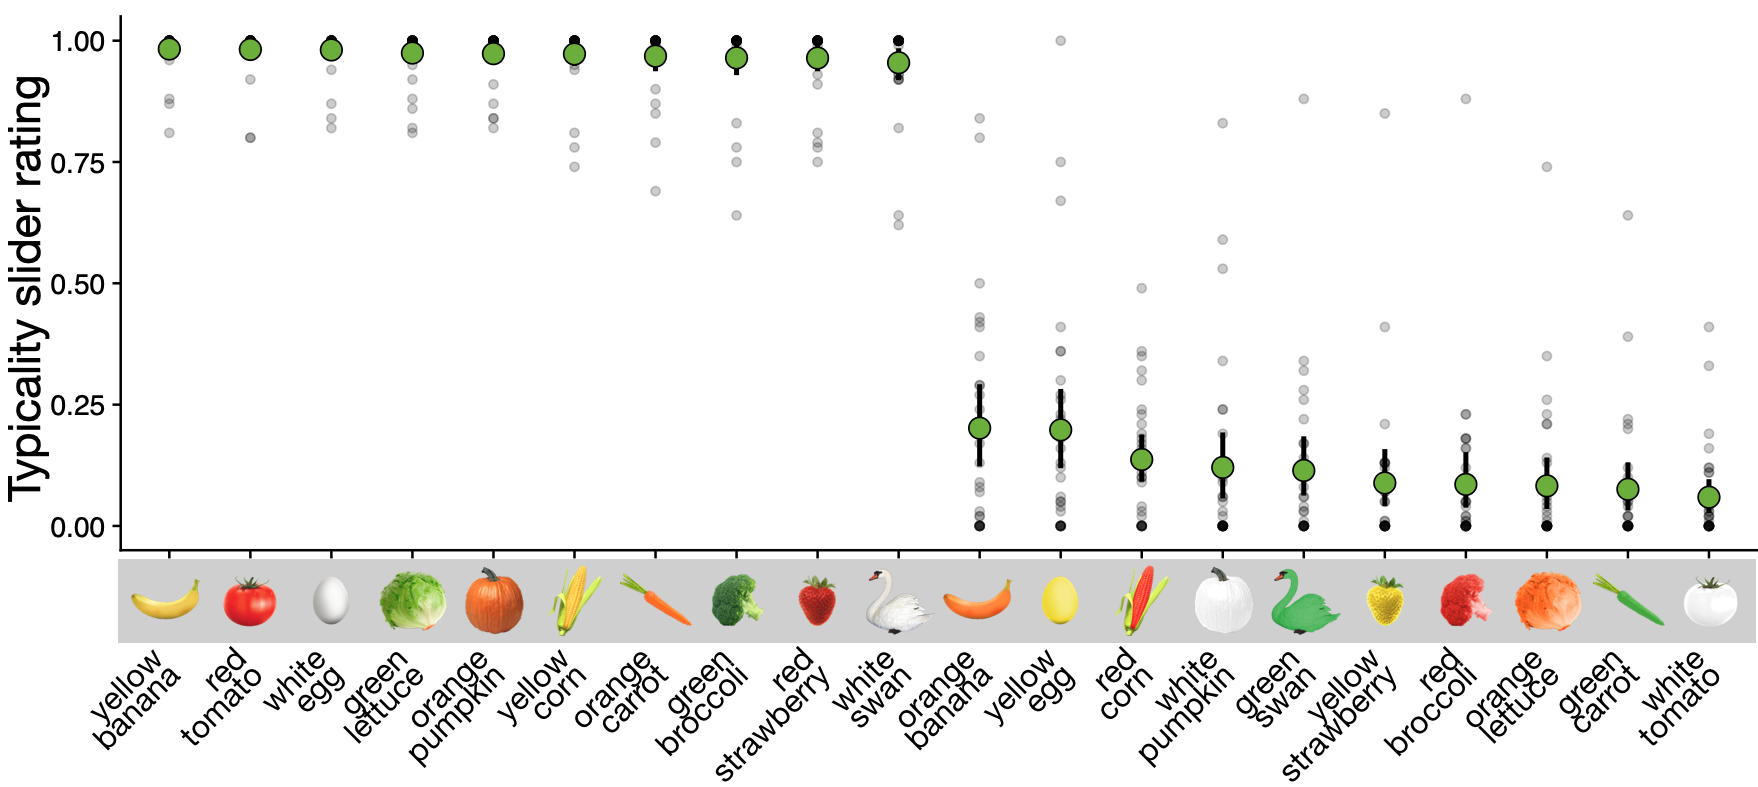
\includegraphics[width=1\linewidth]{img/norming/typicality_results_wimg.png}
	\caption{Final set of stimuli, ordered by typicality. Each object occurs in a typical and atypical color.}
	\label{fig:finalstimuli}
\end{figure}


% \subsubsection{Design}
% Describe the type of design used in the experiment. Specify the variables as well as the levels of these variables. Clearly identify your independent variables, dependent variables, control variables, and any extraneous variables that might influence your results. Explain whether your experiment uses a within-groups or between-groups design.
% For example: "The experiment used a 3x2 between-subjects design. The independent variables were age and understanding of second-order beliefs."

\subsubsection{Procedure}
% The next part of your method section should detail the procedures used in your experiment. Explain what you had participants do, how you collected data, and the order in which steps occurred.
% For example: "An examiner interviewed children individually at their school in one session that lasted 20 minutes on average. The examiner explained to each child that he or she would be told two short stories and that some questions would be asked after each story. All sessions were videotaped so the data could later be coded."
% Keep this subsection concise yet detailed. Explain what you did and how you did it, but do not overwhelm your readers with too much information.

The speaker-listener pairs could communicate freely through a real-time multi-player interface similar to \cite{Hawkins:2015}. The speaker was instructed to communicate a target object out of a four-object context to the listener. The target could be identified by a green border surrounding it. The speaker and the listener saw the same set of objects but in a randomized order to avoid trivial position-based references such as ``the left one''. After the listener clicked on the presumed target, both the speaker and listener received feedback about whether the correct object had been selected.

\begin{figure}
	\begin{center}
		\includegraphics[width=.8\textwidth]{img/production/prod-design.pdf}
	\end{center}
\caption{Example display for the interactive reference game (Exp. 1). Both, the speaker (here \textit{Director}) and listener (\textit{Matcher}) see the same four objects but in a scrambled order. Additionally, the speaker sees a green border around one of the objects, marking the intended target which the listener needs to select.} 
\label{prod-design}
\end{figure}

On critical trials, participants saw the critical displays from Exp.~2. The object to be communicated could be either the object that functioned as the target or the object that functioned as the competitor in that display in Exp.~2, as exemplified in \figref{prod-design}. We continue to refer to `target' and `competitor' in the reporting of this experiment, terms which refer to the function of the object to be communicated in Exp.~2. 
Contexts varied in the typicality of the target and the competitor and the presence of a contrast, resulting in eight conditions. Participants saw each context exactly once. 
Throughout the experiment, half of the critical trials required the speaker to communicate the `target' and in the other half the `competitor'.

In contexts where the contrast was absent, the distinction between target and competitor was meaningless and thus one of the color competitor objects was arbitrarily coded as the target and the other as the competitor. Fillers were eight randomly created contexts where the `contrast' or the `distractor' from \ek{context-ref} was the object to be communicated. Overall, each dyad saw 60 contexts (32 critical trials) in randomized order.

\subsubsection{Data pre-processing and exclusion}

\ek{update numbers} Exclusions were performed on the 141 speakers, since they provided the utterances. Participants were excluded when they participated multiple times in the experiment (1 participant; 139 pairs remaining) and when they did not use a noun from the display in at least half of the cases (27 participants; 112 pairs remaining). These participants clearly misunderstood the task, using expressions such as \textit{yellow monkey} instead of \textit{yellow banana}, or \textit{should be yellow, must have teeth to eat} for \textit{corn}. All speakers indicated that their native language was English.

\subsection{Results}

We excluded two dyads because of multiple participation and 27 dyads for primarily using playful descriptions, e.g., \textit{should be yellow, must have teeth to eat} for the \textit{red corn} object, which left 112 dyads for the analysis.

\figref{prod-results} shows the proportion of color modifier mentions for the target and competitor in each condition. We conducted a Bayesian mixed effects logistic regression predicting color mention for each item from centered fixed effects of contrast presence, target typicality, and competitor typicality, as well as random by-participant intercepts (the most complex random effects structure that allowed the model to converge). 

There was strong evidence of contrast presence ($E=5.25,\ CI=[4.82, 5.69]$), such that when a contrast to the object was present (e.g., another banana, see target proportions in the upper row in \figref{prod-results}), participants were more likely to mention the color modifier than in the absence of a contrast (see target proportions in the lower row in \figref{prod-results} and competitor proportions overall). This was especially true when the object was atypical\footnote{A full interaction model did not converge because color was \emph{always} mentioned in the contrast-present condition with atypical targets, which did not allow the model to generate estimates for interactions involving these conditions. We did not find evidence for any other interactions.}. There was also strong evidence for the object's typicality ($E=2.82,\ CI=[2.52, 3.12]$), such that participants were more likely to include a color modifier when referring to an atypical object than a typical one.

\begin{figure}[H]
	\begin{center}
		\includegraphics[width=.8\textwidth]{img/production/prod-bycond-paper.pdf}
	\end{center}
\caption{Proportion of modifier mentions in each condition for objects that functioned as target and competitor in Exp.~2. Error bars indicate 95\% bootstrapped confidence intervals.} 
\label{prod-results}
\end{figure}

The results of this production experiment show that the probability of a speaker's modifier use is modulated by an object's color typicality, replicating previous results \cite{Westerbeek:2015}. 
\ek{Do other contrastive inference accounts really assume that though?:} The results also confirm the assumption made by many contrastive inference studies that speakers are more likely to produce the color modifier in the presence of a contrast \cite{Aparicio:2018,Grodner:2011,Sedivy:1999}, though this probability is modulated by the typicality of the object.
% Our experiment therefore successfully manipulates the modifier production probabilities a listener can expect in different contexts.

\section{Model predictions}

The production data in \figref{prod-results} were used to obtain RSA model predictions of target preference and we compare these with four variants of the contrastive-function account. Since the assumptions around the contrastive-function account are generally not explicitly formulated, we decided on four variants which represent the foundation of the account (i.e., \emph{vanilla} and \emph{default}), or are relevant possible extensions (i.e., \emph{descriptive inference} extensions). All variants assume that contrastive functions of adjectives are separate from their descriptive form and that the contrastive use is the more informative choice. Consequently, all of these accounts predict all-or-none elicitations of (contrastive) inference: either the target is preferred or there is no preference. While recent work on contrastive inference has started to investigate variation in contrastive inference data \citep{Aparicio:2018,Rubio-Fernandez:2019}, this has so far only addressed variation between adjective classes and has been explained by other aspects than the size of inference itself (e.g., through visual salience of the property).

\figref{model-predictions} displays the predictions contrastive-function accounts and an RSA model of contrastive inference make when varying target typicality, competitor typicality, and contrast presence. It shows the predictions on how likely the listener considers the target object to be the intended referent after observing the modifier (e.g., ``the yellow...''). If neither target nor competitor are preferred, the predicted target consideration is 0.5. If the target is preferred over the competitor, this value increases (and vice versa).

\begin{figure}
	\begin{center}
		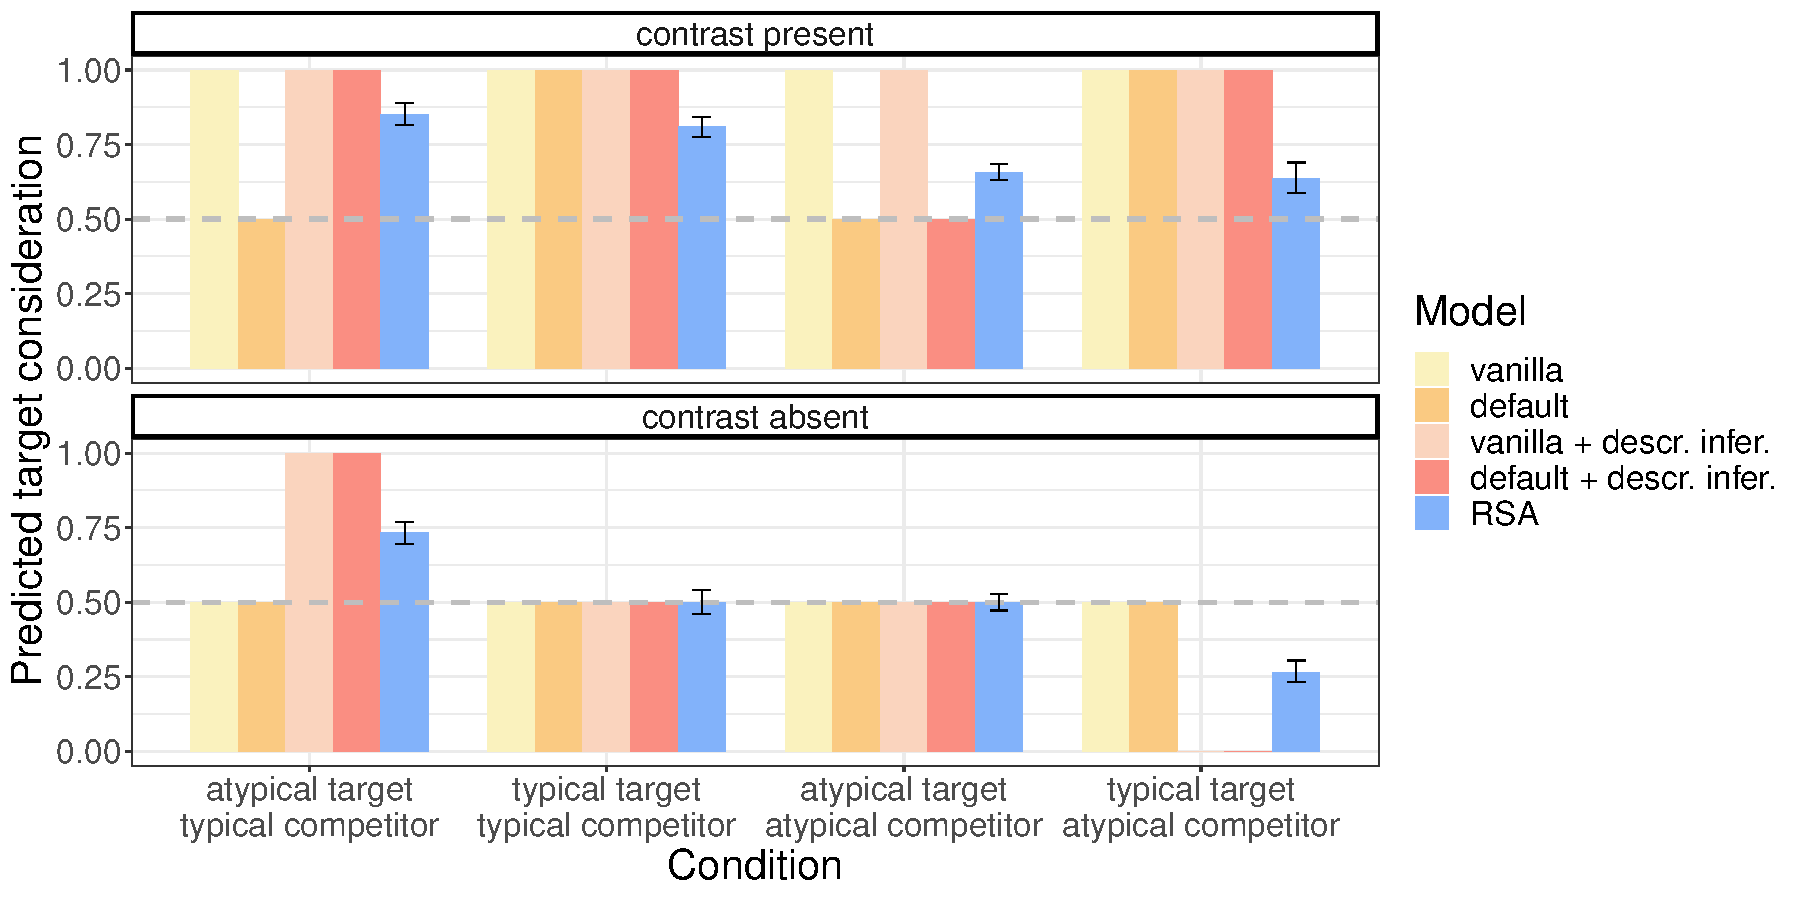
\includegraphics[width=1\textwidth]{img/model-comparison.pdf}
	\end{center}
\caption{Predictions of contrastive function accounts vs. RSA account. Plotted are the probabilities how likely the target object is considered as the intended referent upon observing "the yellow\dots". 1 -(minus) target preference/consideration corresponds to competitor consideration which is not displayed here. \ek{neither blackandwhite nor redgreenblind friendly}} 
\label{model-predictions}
\end{figure}

Firstly, we discuss the four variants of the contrastive-function account.
% \subsection{Contrastive function: vanilla}
The \textbf{vanilla} version simply predicts that an inference only occurs when a contrast is present. This is independent of any properties of the target or the competitor. Consequently, there is no preference when the contrast is absent and a target preference when the contrast is present.\\
% \subsection{Contrastive function: default}
Due to the observation that contrastive inference only appears to arise with objects that don't have color in their \emph{default description}, such as bananas, \cite{Sedivy:2003} proposed the \textbf{default} account. It introduces the restriction to the vanilla account that the contrastive interpretation is only activated if the use of color is surprising given the default description. 
Just like the vanilla account, it uniformly predicts no preference when the contrast is absent. But it only predicts a contrastive interpretation when the target is typical.\\
% \subsection{Contrastive function: vanilla + descriptive inference}
We also consider a variation of the vanilla and default account (displayed in light and darker red respectively in \figref{model-predictions}). In these models, we allow for \textbf{descriptive inference} such that if the speaker uses color in their reference, listeners show a preference for the atypical over the typically colored object. To our knowledge, this version of a contrastive function account has not been discussed in the literature but we believe it's a natural extension. Parallel to the assumption that an adjective's contrastive use is more informative than its descriptive use, the use of the descriptive could be considered more informative than the bare form. Therefore, those models predict a preference for atypical objects when observing the modifier. However this inference only affects the contrast-absent conditions, since it will be overruled by the contrastive interpretation when a contrast is present.

Let's turn to the RSA model predictions. The first most salient difference is the fact that RSA predictions are non-deterministic. While contrastive-function accounts assume a deterministic process on whether an inference arises or not, RSA predicts that listeners can be more or less certain about the speaker's most likely intended referent which is why the strength of target inference varies dependent on the condition. 
In the contrast absent conditions, RSA predicts that listeners prefer the atypical item over the typical one, since speakers are more likely to use the modifier for atypically colored objects. The direction of the preference is most closely related to the \emph{descriptive inference} accounts, since they are also based on this production asymmetry. However those parallels fall apart in the contrast present conditions. Most crucially, the predicted target preference when the competitor is atypical (i.e., in the two right-most conditions) is predicted to be lower than when the competitor is typical. None of the contrastive-function accounts predict a variation in inference (strength) or preference dependent on the competitor typicality.\\
This is the point where the differentiation between \emph{preference} and \emph{contrastive inference} becomes crucial. Consider the right-most condition where the target is typical (e.g., a yellow banana) and the competitor is atypical (e.g., a yellow strawberry). When the contrast (i.e., another banana) is present, the RSA model predicts only a small preference for the target over the competitor, since the speaker could have used the modifier for differentiation or due to the competitor's atypicality. However, there is a strong predicted contrastive inference since the target is predicted to be \emph{dis}preferred in the contrast-absent condition.\\
Reversely, we can consider the left-most condition where the target is atypical and the competitor is typical. Here the model predicts a target preference already in the contrast-absent condition and almost no target boost in the contrast-present condition. This suggests that listeners don't draw a contrastive inference in this condition (that exceeds the atypicality inference), even though there is a preference for the target when a contrast is present.\\
These two cases show the relevance of separating the behavioral pattern of preference in the contrast present condition from the difference in preference matched with the contrast absent condition.

Overall, contrastive-function accounts of contrastive inference make qualitatively and quantitatively different predictions. Most crucially, the RSA model of target preference (1) makes non-deterministic predictions, (2) predicts that listeners draw target inferences even when adjectives are used non-contrastively, and (3) predicts that the nature of the competitor affects target preference.


% \ek{note: contrastive inference is not this thing that arises from a listener realizing that they need to use the contrastive over the descriptive interpretation. It is simply one of many inference changes all originating from very gradient and probabilistic production expectations}

We conducted a comprehension experiment where we elicited listeners' beliefs about the most likely referent given an utterance such as ``the yellow...'' to investigate whether contrastive inference is best explained by assuming contrastive functions of adjectives or a production-centric view of inference in general.





















% \subsection{The theory behind contrastive inference}

% Previous accounts of contrastive inference assume a contrastive function inherent to the adjective which can be activated or not. Any variance observed in the inference data is attributed to perceptual difficulties which are predicted to only occur between adjective classes. We show that a binary contrastive function model (like other form-based accounts) cannot predict the variability of target preference within an adjective class.

% \subsubsection{Default account}

% - CI as a primarily pragmatic process\\
% - Irrespective of adjective class\\
% - Assumption1: adjectives can be interpreted descriptively or contrastively;\\
% - Assumption2: only the contrastive interpretation leads to an inference;\\
% - Assumption3: the contrastive interpretation is only activated when the adjective is not part of the object's default description\\
% - Processing conclusion: listener hears "yellow"; modifier use is descriptive for the competitor, which is why it's irrelevant (see Assumption2); for the target: when a contrast is present and the adjective is not part of the object's \textit{default description}, contrastive interpretation "kicks in", leading to a preference of the target over the competitor\\
% - Given Assumption2, the no-contrast baseline is always uniform and contrastive inference would always be born out by target preference\\
% - In its basic form: all-or-none predictions; might be extendable to include uncertainty about which interpretation should be applied but this account can't make quantitative predictions when these uncertainties should arise

% \subsubsection{Aparicio \& RF}

% - Agree with basic principle of informativity and contrastive function (I believe)\\
% - But attribute all variation to between-adjective-class differences (salience; overinformativity;...)\\
% -> they therefore don't predict any variability within adjective class (\cite{Aparicio:2018} does mention that color might behave different than size for some reason)\\
% - no acknowledgment that "descriptive" inference can interfere with patterns you find

% \subsubsection{Our account}

% - Since the first investigations of this phenomenon, we now have computational tools to predict pragmatic inferences in general. Specifically we propose an incremental adaptation couched within the Rational Speech Act framework \citep{Frank:2012,Goodman:2016,Franke:2009}.\\
% - Speaker and listener reason about each other; therefore listener only has access to production probabilities -> like in Default account, predictions are irrespective of adjective class\\
% - makes quantitative predictions\\
% - In contrast to default account, the model doesn't distinguish between descriptive and contrastive uses, but simply predicts interpretation based on expected use of color modification; in other words cases that previously fell into the category of descriptive use, could also cause inference\\
% - The use of adjectives has been shown to affect interpretation when used contrastively, redundantly, overinformatively,... \\
% - We therefore collapse all assumptions to: interpretation is dependent on production expectation\\
% - This makes new predictions: \\
% - 1) descriptive adjective use can cause inference -> baseline no-contrast condition does not need to be uniform\\
% - 2) the competitor matters since expected descriptive color use for the competitor will interfere with expected contrastive color use -> target preference and contrastive inference strength can vary\\
% - 3) the target matters since on the behavioral side target preference due to expected descriptive use cannot be differentiated from expected contrastive use -> baseline no-contrast becomes crucial to single out contrastive inference strength\\
% - 4) no target preference when a contrast is present doesn't mean the absence of a contrastive inference but might simply be due to a non-uniform baseline no-contrast condition\\
% \ek{addresses: how do we draw inferences? Sedivy still assumes two lexical functions associated with each adjective and noun; we can simplify and at the same time generalize that to simple rational inference on the basis of expectations}
% \ek{given our methodological restrictions (binary choice): we cannot differentiate between binary threshold variance (draw inference or not), or an inherent probabilistic process}



% This makes sense in simplified terms and when we consider the original assumptions behind the \emph{contrast effect} \citep{Sedivy:1999}. Adjectives were/are generally assumed to either bear a \emph{contrastive} role, as in the case of contrasting a tall glass with a small glass, or a \emph{descriptive} role, which would for instance be used to refer to an object in isolation. When contrastive inference was first introduced as a pragmatic phenomenon, it was still assumed that a descriptive use of an adjective could not result in any pragmatic inference. This is the origin of the assumption that there is no preference in the baseline (no-contrast) condition. 
% Provided this is true, any inference that leads us to now consider the target over the competitor as the intended referent is born out as a behavioral preference of the target. However we consider it crucial to differentiate between the preference of the target over the competitor and the boost in target preference compared to the contrast-absent condition. We will show that this distinction is essential for talking about and investigating contrastive inference. 
% To do so, we firstly provide empirical evidence that non-contrastive adjective use leads to pragmatic inferences and therefore changes in the baseline (no-contrast) distribution. But if adjectives can simply take on a contrastive role which overturns the descriptive when a contrast is present, this would still result in uniform target preference behavior, independent of the baseline (i.e., assumption that if it's elicited, CI arises in full). We provide empirical evidence against this assumption by showing that the contrast-absent condition predicts the size of preference when a contrast is present. This clearly suggests that descriptive and contrastive interpretations interfere with each other (e.g., boost from ttp to atp). We therefore argue against a binary treatment of adjectives fulfilling contrastive vs. descriptive roles.
% This also opens the door for variability in contrastive inference strength\ek{add evidence that pragmatic inference strength varies as in \cite{Degen:2015}}. Though previous accounts have acknowledged the variability of contrastive inference strength \citep{Rubio-Fernandez:2019}\footnote{\cite{Aparicio:2016} only acknowledges timing differences, not differences in strength of inference}, it is primarily attributed to between-adjective-class differentiability. We argue that even within the color domain, contrastive inference strength can vary due to \ek{...}.
% If contrastive inference is pragmatic in nature and not simply lexical (i.e., descriptive vs contrastive), and noncontrastive adjective use also results in pragmatic inferences, this suddenly puts the focus on the competitor. 
% Previous accounts of contrastive inference have generally disregarded the nature of the competitor because there was no theoretical motivation to consider it\footnote{Exception in the original size experiment in \cite{Sedivy:1999} where the competitor was for instance taller than the glass but not tall for a pitcher, which makes it kind of similar to typical color competitors here}. For \cite{Sedivy:2003} the competitor is irrelevant because she assumes that the noncontrastive use of adjectives does not result in an inference. She therefore puts a lot of attention to the identity of the target which will affect whether the contrastive function gets activated. This is why she uses typical color-diagnostic targets and non-color-diagnostic competitors. However she notes in footnote 5 that she actually finds a significant listener preference of the competitor over the target when no contrast is present, suggesting that the competitor is a priori more inferred than the target upon hearing the adjective.
% Other accounts such as \cite{Aparicio:2018,Rubio-Fernandez:2019} simply do not address variance within adjective classes and attribute all differences to properties of the adjectives themselves, such as visual salience.
% We show variance of target preference and therefore contrastive inference patterns within the color domain, as \cite{Sedivy:2003} did, and we show that this variance can be explained by production expectations.







\section{Comprehension experiment}\label{sec:exp2comp-noprior}

To investigate which object listeners consider to be the most likely referent after observing the color adjective, we conducted an incremental decision task \cite{Qing:2018}. This is an offline task that allows for eliciting participants' belief distributions at multiple points in the unfolding referring expression. 

\subsection{Method}
% Past tense.
% Be descriptive. Provide enough detail that another researcher could replicate your experiment, but focus on brevity. Avoid unnecessary detail that is not relevant to the outcome of the experiment.
% Make connections. Read through each section of your paper for agreement with other sections. If you mention procedures in the method section, these elements should be discussed in the results and discussion sections.

% \subsection{Method considerations}

Methodologically, contrastive inference behavior has generally been investigated in eyetracking experiments \citep{Sedivy:1999,Ryskin:2019,Aparicio:2016,Rubio-Fernandez:2019,Grodner:2011,Heller:2008}. A contrastive effect is considered to be present if the target preference arises earlier in the contrast condition than in the no-contrast condition. In this paradigm, target preference is approximated by the number of looks to the target (over looks to the competitor). This linking hypothesis has recently been called into question \citep{Qing:2018}. While explicit belief about the intended referent appears to be correlated with an increased proportion of looks, this correlation decreases when the adjective is unexpected \citep{Qing:2018} \ek{more examples!}.\\ 
% Perhaps due to the lack of clear linking hypotheses from eyetracking data to preference, strength of target or contrastive inference is rarely discussed. \cite{Rubio-Fernandez:2019} find differences between adjective classes in increased target and decreased competitor looks upon hearing the adjective. They attribute these differences to properties of \ek{the visual search itself (and lexical properties), rather than the underlying inference size}. \cite{Aparicio:2016} make arguments based on earlier or later emergence of preference but explain this by visual difficulty and not a gradient notion of contrastive/target inference strength. The most intuitive measure of contrastive inference strength could be linked to size of target over competitor advantage, but here again, the concrete linking hypothesis in unclear. As explained in \cite{Rubio-Fernandez:2019}, increased looks to the competitor could as well be due to \ek{...}.\\
% \ek{Can eyetracking be used as a method for prior manipulation experiments (i.e., where the preadjective baseline is non-uniform)?}\\
Recently, those offline measures of preference have gained wider popularity \citep{Qing:2018,Kronmuller:2014, Alsop:2018}. In an \emph{incremental decision task}, the utterance is revealed word-by-word to the listener, who makes an explicit guess about the most likely referent at each step. \citeauthor{Qing:2018} therefore argue that their method offers a more direct window into listeners' beliefs. 
% DISCUSSION?: However each individual response is only a binary signal of either selecting or not selecting the target object and is therefore less rich than the gradient signal from eyetracking experiments. On their own, the results can be interpreted as a binary process where the obtained mean is the mean probability of the threshold between target inference vs non-target inference selection (like randomly sampling a speaker message from the underlying distribution that either does or does not contain the modifier), or the value reflects a sample of each individual's belief distribution which is itself gradient); 
In this paradigm, contrastive inference is the average difference in target preference between the contrast and no-contrast condition in the adjective window. In contrast to the eyetracking methodology, the strength of the inference can easily be translated to the increase in target preference.\\
Due to the more intuitive interpretability and easier data collection procedure, we investigate target preference patterns using the incremental decision task. This paper provides further evidence that the incremental decision task can be used to elicit contrastive inference.
\ek{Can eyetracking be used as a method for prior manipulation experiments (i.e., where the preadjective baseline is non-uniform)?}


\subsubsection{Participants}
% who?, how many?, how selected (random?)?
% basic demographic characteristics of your participants (such as sex, age, ethnicity, or religion), the population from which your participants were drawn, and any restrictions on your pool of participants
% how many participants were assigned to each condition and how they were assigned to each group. 


% \footnote{The experiment was preregistered on \texttt{https://osf.io/27dn8}.}% Originally, we recruited 80 participants and then ran a follow-up with 140 more to get enough data for the evaluation of the RSA model. The results from the first 80 participants do not differ from the full data set, which is why we present them collapsed.}. Each of them were paid \$1.80 for their participation (10\$-16\$/hr). The same restrictions for participation applied as in Exp.~1. 


We recruited 239 participants over Amazon's Mechanical Turk, 121 of which saw atypical color competitors and 118 saw typical color competitors in the critical trials\footnote{The experiment was preregistered on \texttt{https://osf.io/27dn8}. Originally, we recruited 80 participants and then ran a follow-up with 140 more to get enough data for the evaluation of the RSA model. The results from the first 80 participants do not differ from the full data set, which is why we present them collapsed.}. Each of them were paid \$1.80 for their participation (10\$-16\$/hr). We restricted participation to workers with IP addresses in the US and an approval rate of previous work above 97\%. 
27 participants were excluded because they indicated that they did the experiment incorrectly, English was not their native language, or they gave more than 20\% erroneous responses\footnote{An erroneous response is defined as a selection of a non-target object after observing the fully disambiguating noun.}. 211 participants remain, 108 of which were in the atypical competitor and 103 were in the typical competitor condition. 



% We recruited 239 participants over Amazon's Mechanical Turk. 

\subsubsection{Materials}
% Describe materials, measures, equipment, or stimuli used. BRMS!

The critical displays were identical to the critical displays in Exp.~1. 

\subsubsection{Procedure}
% Explain what you had participants do, how you collected data, and the order in which steps occurred.
% For example: "An examiner interviewed children individually at their school in one session that lasted 20 minutes on average. The examiner explained to each child that he or she would be told two short stories and that some questions would be asked after each story. All sessions were videotaped so the data could later be coded."
% Keep this subsection concise yet detailed. Explain what you did and how you did it, but do not overwhelm your readers with too much information.

This experiment was a one-player comprehension-only adaptation of the production study described above and was implemented as an incremental decision task \cite{Qing:2018}: Participants read sentences of the form ``Click on the yellow banana'', which contained a referring expression, and their task was to select the target in the display. Crucially, the sentence was only gradually revealed. Participants made a selection at each of three time points: (1) before receiving any information about the referent (i.e, after observing ``Click on the'', \emph{prior window}), (2) after observing the adjective (``Click on the yellow''), \emph{adjective window}, and (3) after observing the full referring expression with the disambiguating noun (``Click on the yellow banana''), \emph{noun window}. 

To center the position of the mouse after each selection, a button appeared in the center of the grid which had to be clicked to reveal the next word or to advance to the next trial. 

\ek{The data from before adjective onset we use to estimate the prior distribution. For cleaner effects, we don't use the data from this experiment to investigate post-adj selections due to a strong non-switching bias. The results presented here are from the post-adj-only experiments}

Target typicality and contrast presence were within-participant manipulations, competitor typicality was a between-participants manipulation
\footnote{The complexity of the 2x2x2 design and considerations of power required that either the number of trials per participant  be high or one manipulation  be between-participants. We decided for a smaller number of trials to minimize the probability of strategic responses or response fatigue developing over the course of the experiment. Contrast presence and target typicality could not be manipulated between-participants since these regularities are easily detectable by a participant within an experiment. Between-participants manipulations are considered more conservative \cite{Charness:2012} and random by-participant intercepts and slopes were included in the analyses to account for random by-participant variability.}
. All critical trials used color modified referring expressions. 
Filler trials were included that primarily used unmodified utterances and referred to one of the other three items in the display to avoid learning effects. 
Participants completed 55 trials (20 critical) in random order. To minimize the risk that the speaker was perceived as pragmatically uncooperative \cite{Grodner:2011,Pogue:2016,Ryskin:2019}, trials with modified utterances that referred to a typical object with no contrast only appeared after the 15th trial. To familiarize participants with the task, they first completed four practice trials in the director role.
% Participants completed 55 trials (20 critical) that were randomized with the only restriction that modified utterances that referred to a typical object with no contrast only appeared after the 15th trial to minimize the risk that the speaker was perceived as pragmatically uncooperative \cite{Grodner:2011}. To familiarize participants with the task, they first completed four practice from the director's perspective.
 


\begin{figure}
	\begin{center}
		\includegraphics[width=.5\textwidth]{img/comprehension/IDT-design.pdf}
	\end{center}
\caption{Design of the incremental decision task. The referring expression was placed above the grid and revealed gradually. After each new word participants made a selection indicating their best guess about the intended target.} 
\label{IDT-design}
\end{figure}


\subsubsection{Data pre-processing and exclusion}
% We excluded participants due to multiple participation (1), self-reported confusion about the experiment (13), self-reported non-English native language (6), and a higher than 20\% error rate\footnote{An incorrect response is defined as a selection of a non-target object after observing the fully disambiguating noun.} (7).
% 211 participants remained; 108 saw atypical and 103 saw typical competitors on critical trials. 

We excluded participants who did the Hit multiple times (1), who indicated that they did the Hit incorrectly or were confused (13), who indicated that they had a native language other than English (6), and who gave more then 20\% erroneous responses (7). An incorrect response is defined as a click to a non-target object after observing the fully disambiguating noun, i.e., participants are excluded who selected the wrong final object more than 11 times. Overall, we excluded 27 people, which is 11\% of the subjects. 211 participants remain, 108 of which were in the atypical competitor and 103 were in the typical competitor condition. 

\subsection{Results}

\ek{modelcompr-results} shows the proportion of target and competitor selections in the adjective window (lighter colors) alongside the RSA model predictions derived from the Exp.~1 production probabilities (darker colors), grouped by condition.\footnote{Neither of the other two objects in the display was chosen after observing the adjective.} %First, we focus on the empirical results where we predicted that the presence of the contrast and the typicality of the objects will affect the listeners' object choices. 
We conducted a Bayesian mixed effects logistic regression on adjective window choices, predicting the log odds of target over competitor selections from centered fixed effects of contrast presence, target typicality, competitor typicality, and their interactions, prior window selection, as well as the maximal random effects structure that allowed the model to converge\footnote{Random effects: $(1+\text{contrast}*\text{target\_typicality}|\text{participant}) + (1+\text{contrast}*\text{competitor\_typicality}|\text{target}) + (1+\text{contrast}*\text{target\_typicality}|\text{competitor})$}.

There was strong evidence for an effect of contrast presence ($E=0.34,\ CI=[0.13,0.53]$), such that when there was a contrast object (top panels), there was a general preference for target over competitor selections, replicating the standard contrastive inference effect. This preference was largest when the target was atypical and the competitor was typical and disappeared when the target was typical and the competitor was atypical, following the qualitative predictions discussed in the modeling section above and exemplified in \ek{example-context}. There was also strong evidence for an effect of competitor typicality ($E=-0.54,\ CI=[-0.90,-0.17]$), such that when the competitor was atypical, target selections decreased, which is again in line with our predictions.

% When there was no contrast (bottom panels in \figref{modelcompr-results}) and target and competitor differed in typicality, there was a preference for the object with the atypical color. When the two objects were similarly (a)typical, participants showed no preference for one over the other, again in line with the qualitative predictions.

% Before an adjective is observed, all items should appear equally likely to be the target, which is supported by the generally uniform distribution in all conditions. After the adjective is revealed (darker colors), only the target and competitor are legible options and we predicted that the presence of the contrast and the typicality of the objects will affect the listeners' object choices.

\begin{figure}
	\begin{center}
		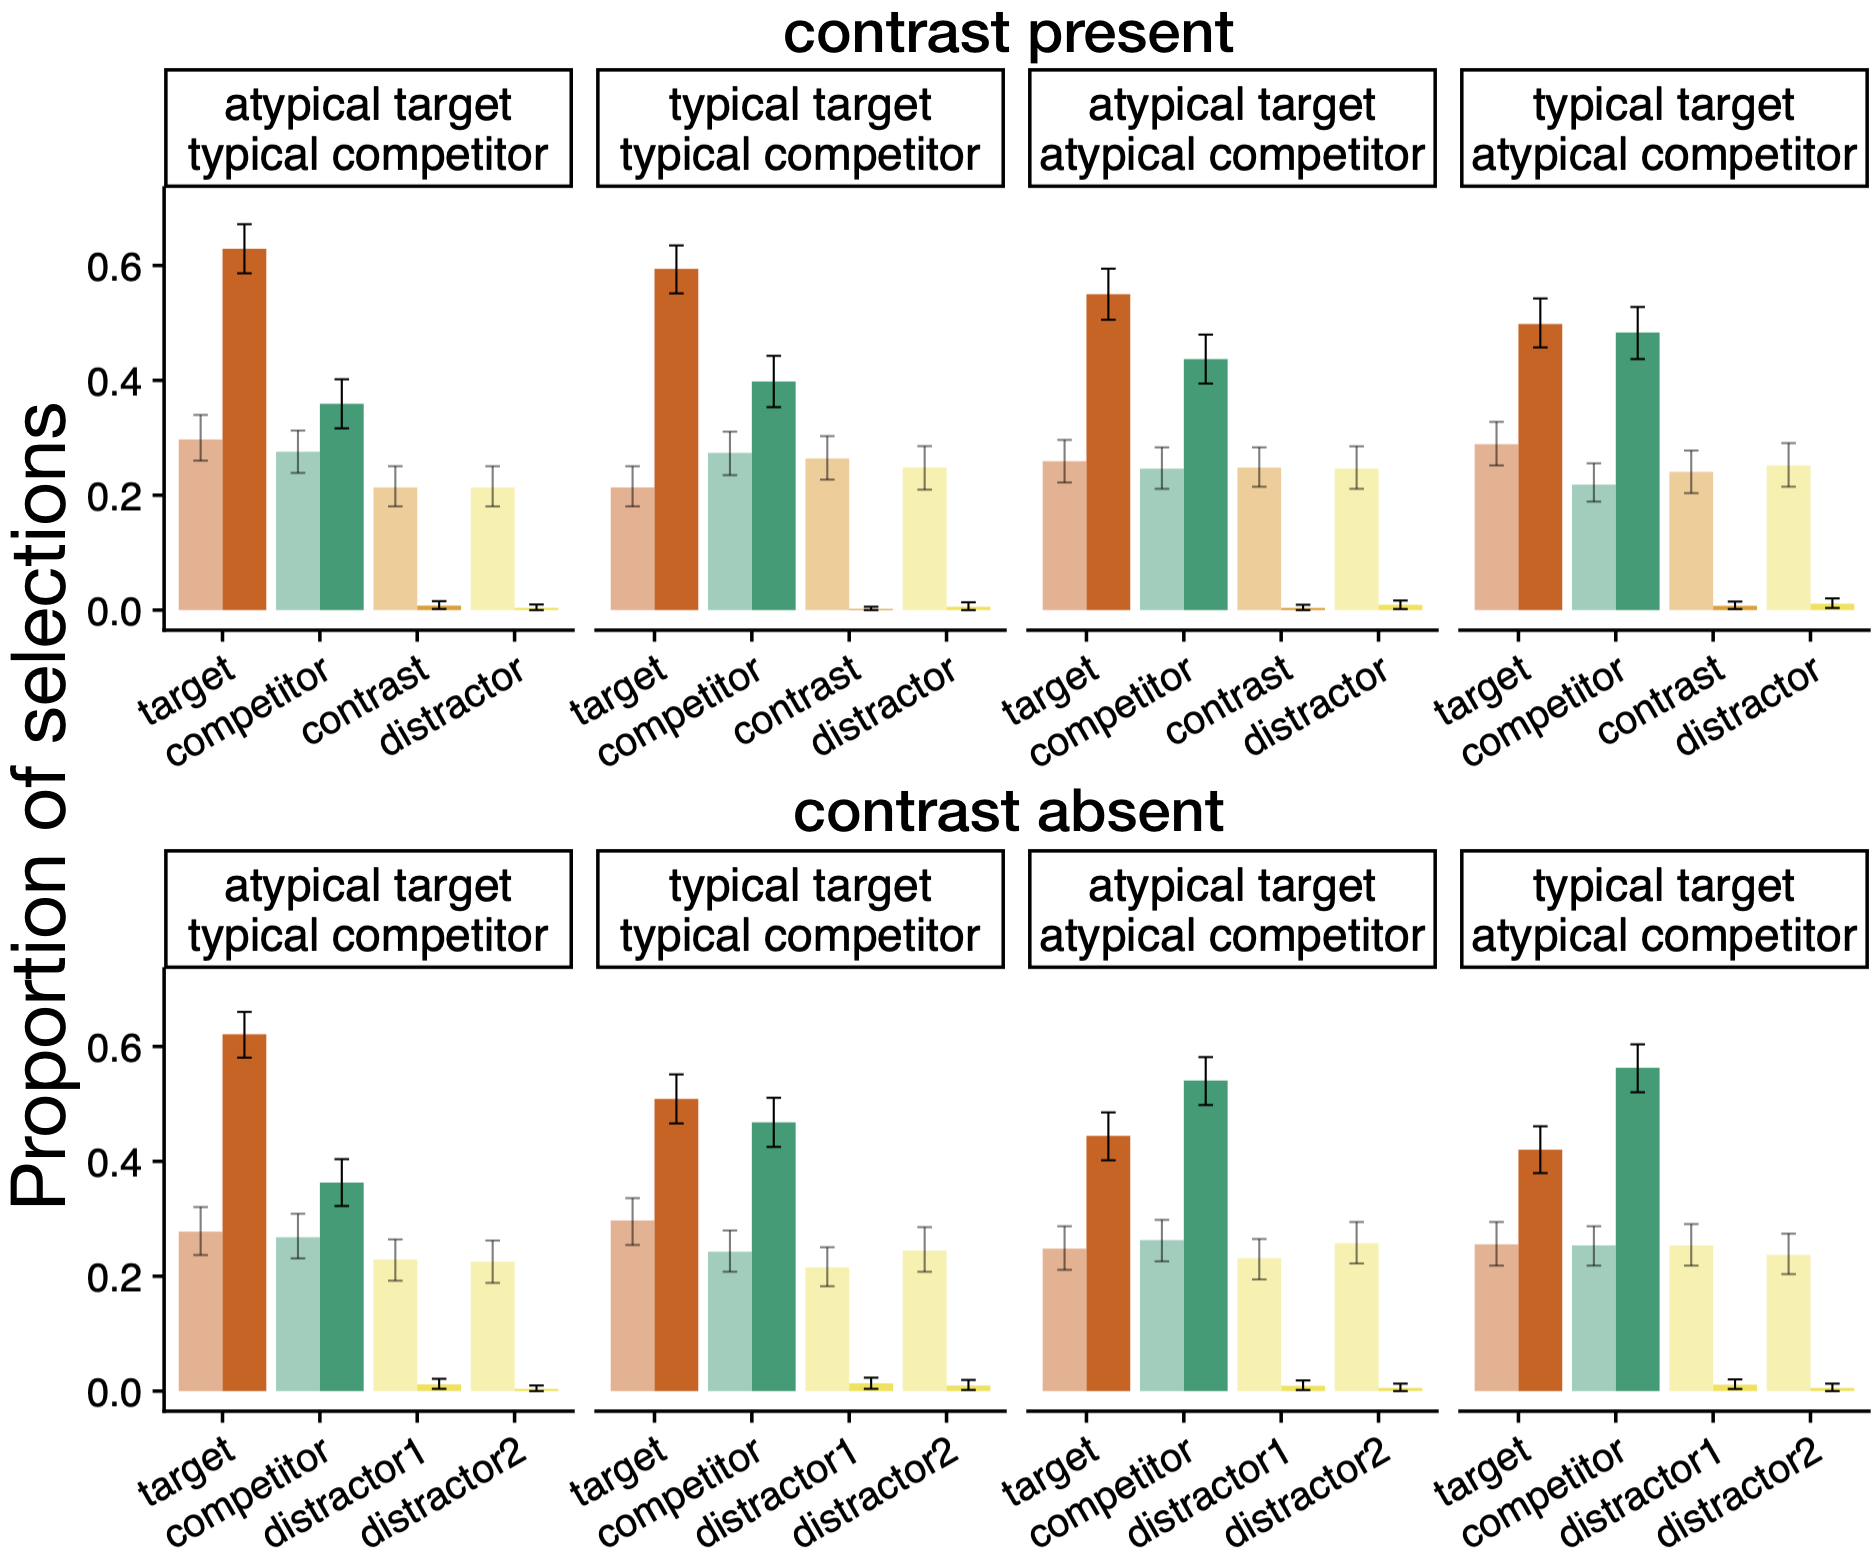
\includegraphics[width=1\textwidth]{img/comprehension/compr-results.png}
	\end{center}
\caption{Results for the comprehension study, showing the proportion of selections for each item in the display and each condition. The bars in lighter colors indicate the selections before, the darker bars are the selections after the adjective was observed. Error bars are 95\% bootstrapped confidence intervals.} 
\label{compr-results}
\end{figure}

% \begin{figure}
% 	\begin{center}
% 		\includegraphics[width=.475\textwidth]{graphs/model-bycond-paper.pdf}
% 	\end{center}
% \caption{Empirical proportion (light bars) and model predicted probability (dark bars) of object selections in each condition. Dashed line indicates chance. Error bars indicate 95\% bootstrapped confidence intervals.} %for each target-competitor item combination.} 
% \label{modelcompr-results}
% \end{figure}

Although object selections in the prior window were approximately at chance, there was strong evidence that it affected participants' specific selections of their adjective window choices ($E=1.46,\ CI=[1.29,1.63]$). These results suggest that when participants' prior selection is congruent with the newly revealed adjectival information, they stick with their previous choice. 
% This observation will be relevant for later discussions of the size of target preference.
% However the main effects of contrast ($E=0.34,\ CI=[0.14,0.53]$) and competitor typicality ($E=-0.54,\ CI=[-0.90,-0.17]$) still remain.

% Before the adjective was observed, object selections were approximately at chance. However, the selections after reading the adjective were affected by the participant's previous selection, such that a participant who previously selected the competitor was more likely to select the competitor again than switch to the target (and vice versa). But since object selections before the adjective followed a uniform distribution, any patterns that appear after the adjective cannot be an artifact of the reselection bias.

Overall, these results suggest that the color typicality of not just the target, but of competitor objects in the display, too, affects the inferences listeners draw about the intended referent. An atypical competitor alone can promote the competitor over the target when the contrast is absent and can even make the target preference disappear when a contrast is present. %It is therefore highly relevant to control for the quality of the competitor when assessing contrastive inferences. 

If one quantifies contrastive inference as an increased target preference in the adjective window in the contrast-present condition compared to its item-matched contrast-absent condition, the contrastive inferences is small or even non-existent when the target is atypical and the competitor typical (left column of \ek{modelcompr-results}). This may explain why contrastive inferences did not occur with target items of unpredictable colors \cite{Sedivy:2003}. However, even though those items have been reported to have a higher modifier production probability in isolation \cite{Sedivy:2003}, future work still needs to establish how those objects of unpredictable colors relate to (a)typically colored objects.

\section{Model predictions (with prior)}\label{sec:model-noprior}

\section{Comprehension experiment -- prior manipulation}\label{sec:exp2comp-prior}

\subsection{and what other models have to say about that}

\section{Discussion}\label{sec:discussion}

% \subsection{What is the thing we call contrastive inference?}

% \ek{there is target inference and contrastive inference which is the difference of target inference between the contrast conditions}

% phenomenon of target preference as described by Sedivy\\
% \citeauthor{Sedivy:2003} describes the behavioral pattern behind contrastive inference as follows: 
% \begin{quote}
% 	\textit{[T]he target was distinguished from a competitor object [...] more quickly when a contrasting object of the same category was present in the display [...] than when no such contrasting object was present.}
% \end{quote}
% % \ek{assumes uniform baseline; counterargument: tax condition where there is no target preference but still contrastive inference because of non-uniform baseline}
% -> This has since been termed contrastive inference. As a consequence, when we talk about contrastive inference, we usually describe it as a behavioral pattern of preference for the target over a competitor due to the presence of a contrast.\\
% We argue for a more general definition of contrastive inference which defines it as the increased preference of the target over the competitor due to the presence of a contrast. In other words the focus of the definition should not be the behavioral pattern of target preference in the contrast-present condition, but the boost in target preference compared to the no-contrast condition.\\
% baseline distribution is relevant in two cases: in tax there is no target preference but CI, and in atx where there is a target preference but no CI; it's therefore crucial to evaluate contrastive inference always with consideration of the baseline no-contrast condition.

\ek{speaker specific adaptation \citep{Pogue:2016}}
% IDT: However each individual response is only a binary signal of either selecting or not selecting the target object and is therefore less rich than the gradient signal when using eyetracking. On their own, the results can be interpreted as a binary process where the obtained mean is the mean probability of the threshold between target inference vs non-target inference selection (like randomly sampling a speaker message from the underlying distribution that either does or does not contain the modifier), or the value reflects a sample of each individual's belief distribution which is itself gradient); 
\ek{mention that done in English, prenominal, should extend to other languages (connect to that literature)}
\ek{given our methodological restrictions (binary choice): we cannot differentiate between binary threshold variance (draw inference or not), or an inherent probabilistic process}

\section{Conclusion}\label{sec:conclusion}




































\section{Acknowledgments}
QP1 committee, ALPS lab, CAMP, CUNY, CogSci, MagPie team (reference game setup);
Previous versions of this work have been presented at CogSci, CAMP and CUNY

\appendix


\section{Norming}\label{sec:norming}

The items used in the experiment were carefully selected according to the results of four norming studies. 
First of all, the objects needed to be color-diagnostic (Section \ek{coldiagnorming}), since those objects show the highest difference in color modifier use dependent on their color typicality \citep{Westerbeek:2015,Tanaka:1999,Sedivy:2003}, our central manipulation. In addition, the items needed to be shape-diagnostic, such that they would still be recognizable when presented in a non-prototypical color. Plums, oranges, limes and lemons for example are objects with low shape-diagnosticity and are therefore hard to identify when presented in an atypical color (Section \ek{freeprodnorming}). Furthermore the items needed to be easily recognizable and nameable (Section \ek{nameabilitynorming} and \ek{freeprodnorming}). Previous literature suggests that unexpected utterances and labels might be a confound in eyetracking experiments \citep{Qing:2018}. To make the items further suitable for eyetracking studies, target and color competitor were never cohort competitors of each other (e.g., \cite{Cole:1980}, \cite{Marslen-Wilson:1984}), i.e., they were always distinguishable at noun onset.

Furthermore, to our knowledge, previous experiments which manipulated the color typicality of objects did not counterbalance the colors used for typical and atypical instances. Certain colors (e.g., blue) primarily occurred as an atypical instance while other colors (e.g., green) occurred as a typical one. However, color hues vary in their a priori preference and elicit different emotional responses (see \cite{Palmer:2013, Elliot:2014} for reviews on color preference and psychology). The color hue imbalance for typical and atypical objects might therefore be a non-negligible confound to the typicality effect. Each color in this data set occurs twice as a typical instance and twice as an atypical instance to counteract this potential confound.

Finally, the typical and atypical instance of each object was normed to ensure that the color manipulation of the images shows the desired difference in typicality ratings (Section \ek{typicalitynorming}).

Since half of the conditions require the target and color competitor both to be (a)typical, we needed two (a)typical instances for each color. Motivated through this experimental design, the final set of stimuli consists of ten color diagnostic objects (each of them in a typical and atypical instantiation), evenly distributed over five colors. To determine the most suitable items, our initial set of potential stimuli comprised six colors (green, orange, pink, red, white, yellow), each with at least four presumably typical color-diagnostic instances (25 items in total).

\begin{figure}
	\includegraphics[width=\linewidth]{img/norming/all_norming_designs.pdf}
	\caption{Norming studies. \ek{possibly remove button}}
	\label{fig:norming-designs}
\end{figure}



In the end, the final set of stimuli comprises 10 objects, each occurring in a typical and atypical color.
Items can occur in the colors yellow, red, green, orange and white. Each color occurs twice as typical and twice as atypical. The objects are \textit{banana, broccoli, carrot, corn, egg, lettuce, pumpkin, strawberry, swan,} and \textit{tomato}. The full set of stimuli is displayed in Figure \ref{fig:finalstimuli}.

% \ek{perceptualfeature}
% The experimental design is adapted from \cite{Tanaka:1999}. 

% Participants were asked to list three perceptual features of an object, which they entered into three free production text boxes. They could proceed to the next trial if they either entered all three features or indicated by ticking a checkbox that they did not know the object.
% An item was considered color-diagnostic if color was mentioned as the first feature, \textbf{and} participants agreed on the specific color the object was associated with. 
% As expected, color was in general more likely to be mentioned for the objects that were intended to be color-diagnostic and less likely for the non-color-diagnostic objects (see Figure \ek{fig:norming1resultsoverall}).

% \ek{even though egg has low rating in first feature, color is almost always mentioned as one of the three features making it the best option given the alternatives.}

% % \begin{figure}
% % 	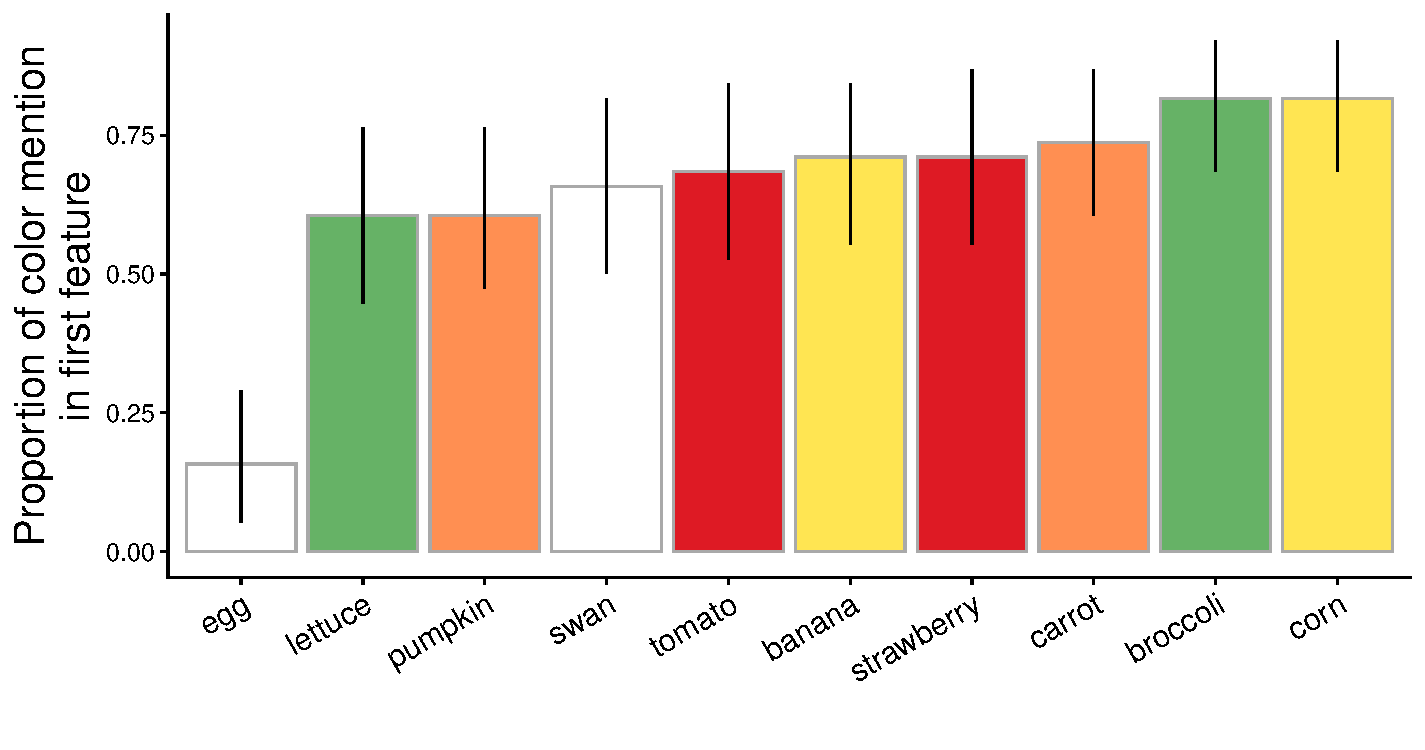
\includegraphics[width=1\linewidth]{img/norming/featurenorming_resultsoverall.pdf}
% % 	\caption{Proportion of color being mentioned as a first perceptual feature for presumably color-diagnostic objects, facetted by the assumed color association. The dotted line marks the point where half of the time, color was mentioned as the first feature.}
% % 	\label{fig:norming1results}
% % \end{figure}

% \begin{figure}
% 	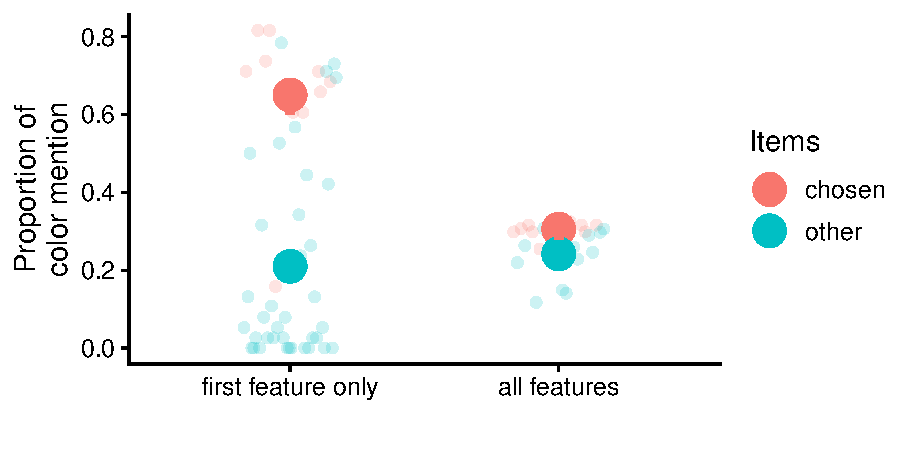
\includegraphics[width=.85\linewidth]{img/norming/featurenorming_resultsnew.pdf}
% 	\caption{Proportion of color being mentioned as a first perceptual feature and among all perceptual features. The final set of stimuli (e.g., \textit{banana} and \textit{swan}) are displayed in red, all other normed items (e.g., \textit{butterfly} and \textit{zucchini}) are in blue.}
% 	\label{fig:norming1resultsnew}
% \end{figure}

% \ek{nameability}
% After we normed for color-diagnosticity, we chose an image depiction for each object and normed them for their nameability. Determining whether an object is nameable served two main purposes. Firstly, we ensured that the dominantly chosen label corresponds to the concept we had normed for in the color-diagnosticity norming (Section \ek{coldiagnorming}). Furthermore, participants should agree on the label that best describes the chosen depiction. Strong agreement among participants is an indication that the noun label can be used reliably. Strong disagreement about the label might affect the production and comprehension of the referring expressions. If speakers are uncertain about an object's property (in this case, its type), they are more likely to overmodify \citep{Horacek:2005, Williams:2017}. Additionally, a listener's surprisal of hearing an unexpected label might affect for instance their fixations in eyetracking experiments, creating a potential confound in the analysis \citep{Qing:2018}.
% We evaluated the results according to how many labels were used. If more than one label was used, we favored cohort competitors (e.g., \textit{bike} and \textit{bicycle} were more acceptable deviations than \textit{traffic cone} and \textit{cone}).

% Overall, participants agreed on the labels, but there were some notable exceptions. Both, the pickle and zucchini, were called \textit{cucumber} to a non-negligible degree. Given that they also have low shape-diagnosticity, both objects were excluded from the final set of stimuli. Other items that received a variety of labels were the traffic cone (e.g., \textit{traffic cone, cone, caution cone, hazard cone}) and the rubber duck (e.g., \textit{rubber duck, duck, duck toy}). These cases were problematic because the labels are not cohort competitors of each other, which makes them crucially distinct in real-time (auditory) setups such as eyetracking experiments.

% \ek{typicality}
% After selecting the most promising objects and creating atypical counterparts, we normed depictions of these items according to their typicality to ensure that they are in fact perceived as typical and atypical. Norming the atypical instances is especially necessary since in fact most of these items occur in different colors in the world. For example, there are red bananas, purple carrots, blue corncobs, yellow tomatoes, varying colors of pumpkins and artificially colored eggs. A successful typicality manipulation should maximize the difference between typical and atypical ratings for each object.

% Each participant saw 45 trials in which they were asked ``How typical is this object for a \textbf{NOUN}'' with a depiction of an object in either its typical or atypical instance, as shown in Figure \ek{fig:norming23design}B, and where \textbf{NOUN} is the established label from the nameability norming experiment. Participants indicated their response on a continuous slider which was initialized in the center of the scale and was underlyingly coded as ranging from 0 to 100.
% For the typicality norming, we selected 11 color-diagnostic objects from the set of the previous norming studies and presented each in their typical color and in one to two atypical colors. 

% Overall, this resulted in 25 color-diagnostic and 20 non-color-diagnostic stimuli. The atypical depictions were created from the typical depictions by changing the typical to an atypical color hue\footnote{The exception to this are the red and yellow strawberries which were both created from a picture of a yellow-green strawberry.}. This means that potential greenery around the item or stems were preserved to maximize the inherent naturalness of the item (as can be seen in the carrot or pumpkin items in Figure \ref{fig:finalstimuli}). 

% We only used the colors of the typical items (i.e., green, orange, red, white, and yellow) for the atypicality manipulation to create a counterbalanced final set of stimuli. Again, the colors were distributed evenly over all objects such that each color occurred as an atypical instance on exactly two objects. 

% In the analysis, we assessed whether the color manipulation of the images showed the desired difference in typicality ratings.

% \begin{figure}
% 	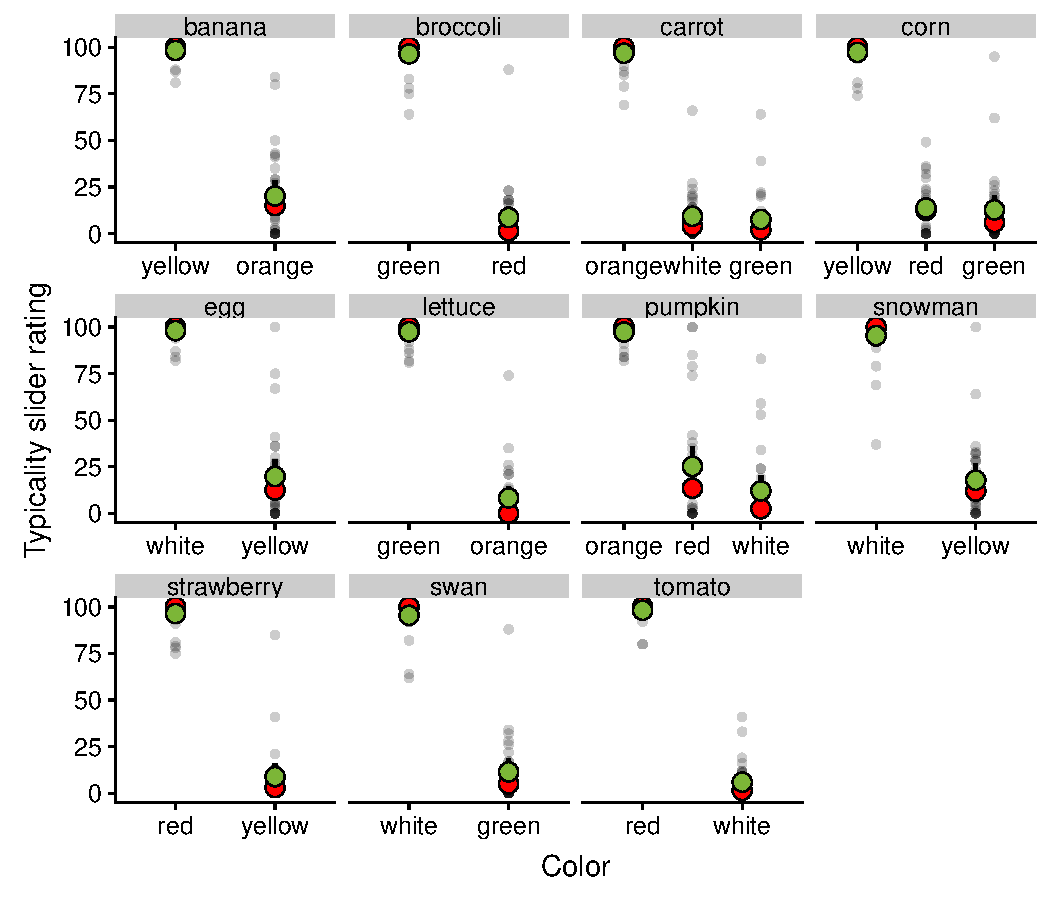
\includegraphics[width=0.9\linewidth]{img/norming/norming3_results.pdf}
% 	\caption{Typicality ratings for differently colored instances of the same object. Higher values indicate higher typicality. Individual data points are in gray, means in green and medians in red.}
% 	\label{fig:norming3results}
% \end{figure}

% As shown in Figure \ref{fig:norming3results}, there generally was a clear distinction between the typical and atypical instances for each object. 

% Of the three items that were normed in two atypical colors (carrot, corn, and pumpkin), the red and white pumpkin showed the biggest difference. Therefore, we chose the white over the red pumpkin, and, following from that, the green carrot and red corn as atypical instances. 
% Finally, even though the egg and snowman received similar ratings for their atypical instance, the white egg is rated slightly more typical than the depiction of the white snowman.

% However we have to note that even though the orange banana is predominantly rated below 50, it is still not as atypical as other items. This might be due to the high similarity between the colors yellow and orange.

% \ek{freeprod}
% Finally, we normed the stimuli chosen from the typicality norming study as to whether those depictions are nameable as intended.
% Participants saw each object exactly once and its typicality was randomized, resulting in 11 critical trials. This was done to prevent convergence effects on a label when the object occurred the second time (e.g., \cite{Clark:1986}). Each participant additionally completed 20 filler trials, where they saw non-color-diagnostic objects.

% \begin{figure}
% 	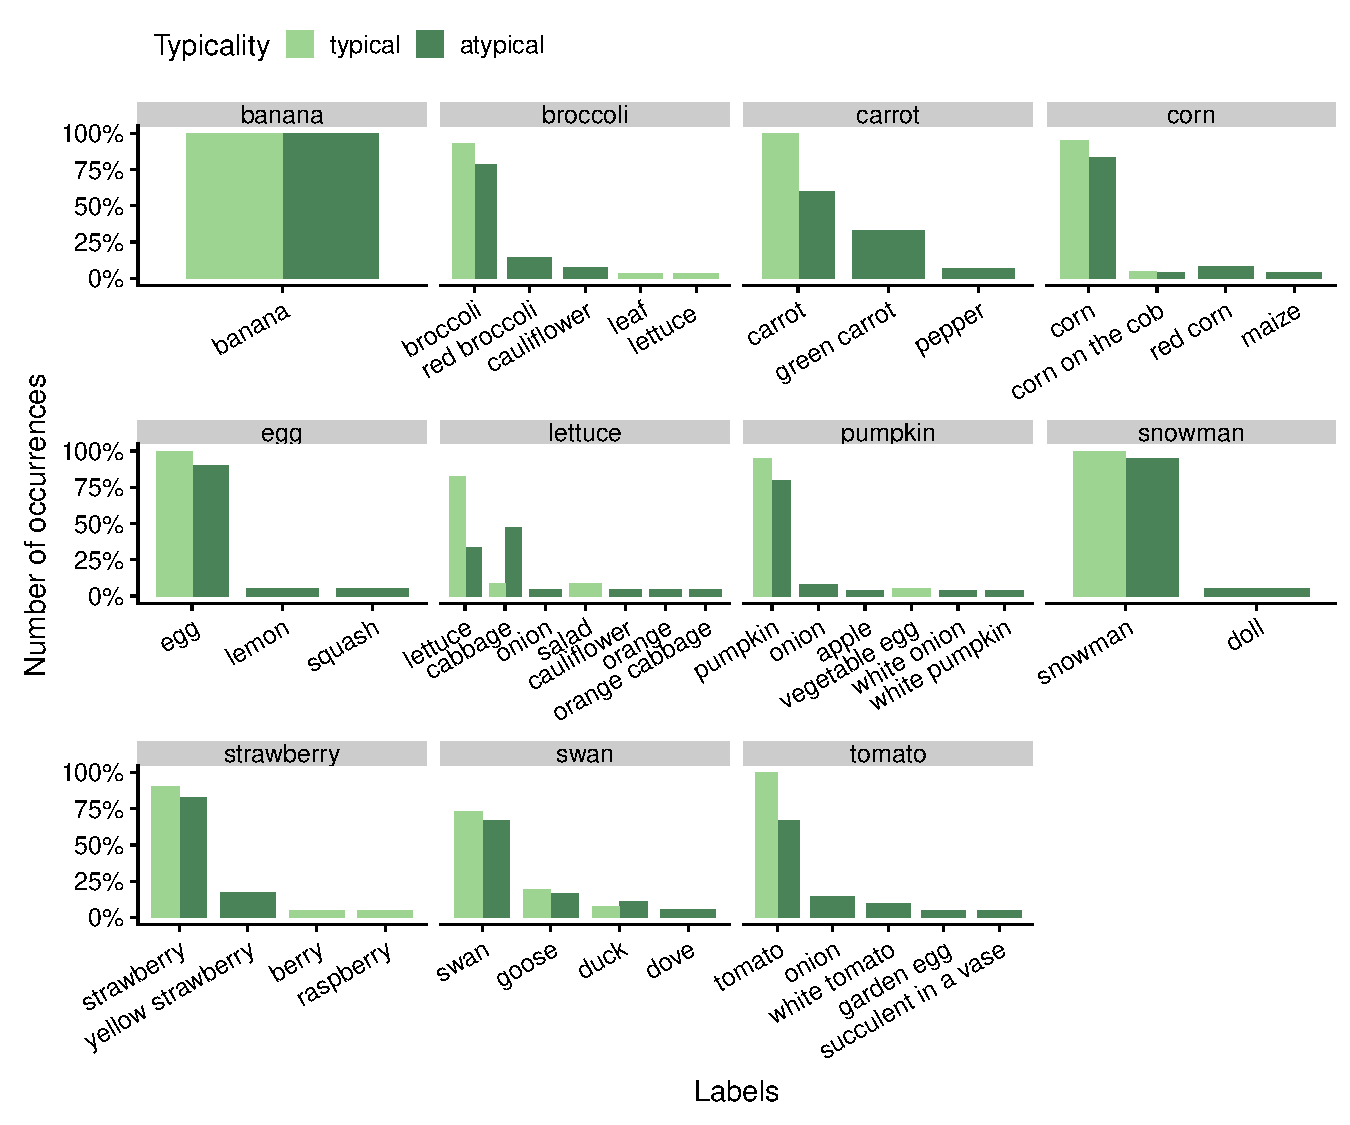
\includegraphics[width=0.9\linewidth]{img/norming/norming4_results.pdf}
% 	\caption{Labels produced for each item in a free production experiment for all remaining stimuli. Labels produced for typical items are in light green, labels produced for their atypical counterparts in dark green.}
% 	\label{fig:norming4results}
% \end{figure}

% As the results in Figure \ref{fig:norming4results} show, participants generally gave the same label to both the atypical and typical instance.


% \ek{Conclusion}



















% \begin{figure}
% 	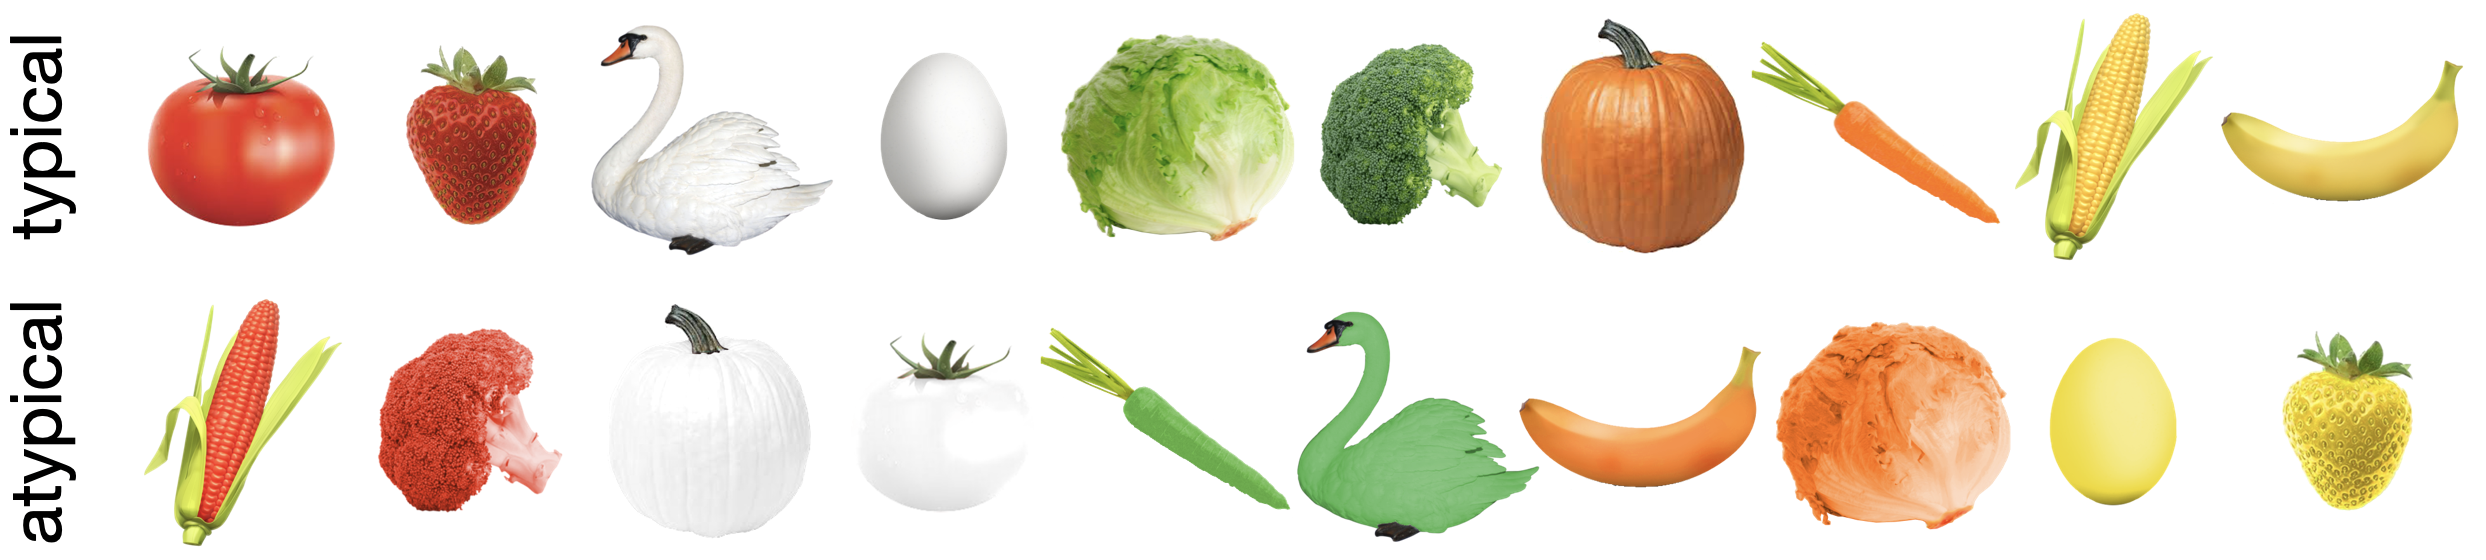
\includegraphics[width=0.6\linewidth]{img/norming/finalstimuli.png}
% 	\caption{Final set of stimuli, ordered by color and typicality. Each object occurs in a typical and atypical color.}
% 	\label{fig:finalstimuli}
% \end{figure}


% \bibliographystyle{apalike}
\bibliography{../../../../../../Dropbox/library/library}


\vfill
\pagebreak

\end{document}

%
% Please see the package documentation for more information
% on the APA6 document class:
%
% http://www.ctan.org/pkg/apa6
%



